\documentclass[aspectratio=169]{beamer}
\usepackage[utf8]{inputenc}

\usetheme{Madrid}
\usecolortheme{default}
\useinnertheme{circles}

\definecolor{Logo1}{rgb}{0.06274509803921569, 0.17254901960784313, 0.32941176470588235} %(16, 44, 84)
\definecolor{Logo2}{rgb}{1.0, 0.5764705882352941, 0.3254901960784314} %(255, 147, 83)

\setbeamercolor*{palette primary}{bg=Logo1, fg=white}
\setbeamercolor*{palette secondary}{bg=Logo2, fg=white}
\setbeamercolor*{palette tertiary}{bg=white, fg=Logo1}
\setbeamercolor*{palette quaternary}{bg=Logo1,fg=white}
\setbeamercolor{structure}{fg=Logo1} % itemize, enumerate, etc
\setbeamercolor{section in toc}{fg=Logo1} % TOC sections
\usepackage{xcolor}
%\usepackage{enumitem}
%------------------------------------------------------------



%------------------------------------------------------------
%This block of code defines the information to appear in the
%Title page
\title[Multi - Classification] %optional
{CLASSIFICAÇÃO MULTICLASSE DE DOENÇAS E PRAGAS EM FOLHAS DE CAFÉ USANDO APRENDIZADO PROFUNDO}

% \subtitle{And its subtitle}

\author[Clécio Elias] % (optional)
{Clécio Elias Silva e Silva}

\institute[UFAC] % (optional)
{
  Centro de Ciências Exatas e Tecnológicas\\
  Universidade Federal do Acre
}

\date[Progresso da Pesqusia] % (optional)
{Progresso da Pesquisa, 2024}


\logo{
\includegraphics[height=.6cm]{ourlogo.png}}

%End of title page configuration block
%------------------------------------------------------------





%------------------------------------------------------------


\begin{document}

%The next statement creates the title page.
\frame{\titlepage}


%---------------------------------------------------------
%This block of code is for the table of contents after
%the title page
\begin{frame}
    \frametitle{Agenda}
    \tableofcontents
\end{frame}
%---------------------------------------------------------
%----------------------------------------------------------------- BEGIN SLIDES ------------------------------------------------------------

\section{Introdução}



%---------------------------------------------------------

\begin{frame}
    \frametitle{Introdução}
    \begin{columns}

        \column{0.5\textwidth}

        Pesquisa anterior e artigo publicado na SBC.

        \column{0.5\textwidth}
        \begin{figure}
            \centering
            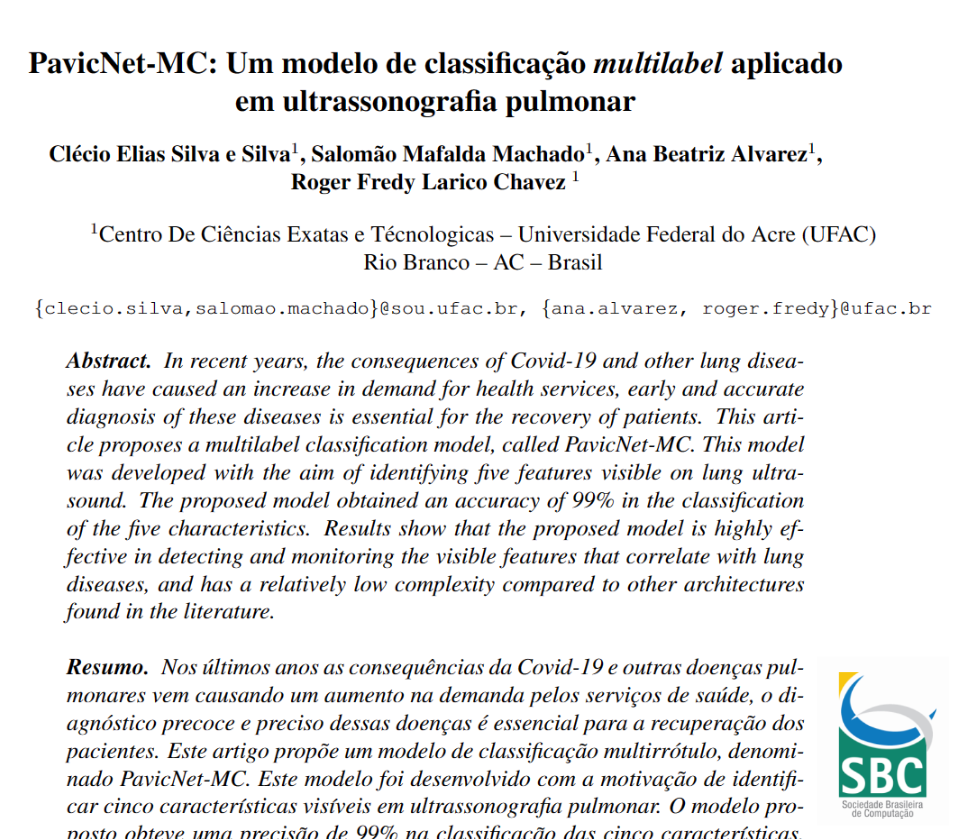
\includegraphics[scale=0.3]{img/Artigo.png}
            %\caption{Caption}
            \label{fig:enter-label}
        \end{figure}


    \end{columns}
\end{frame}

%---------------------------------------------------------

%---------------------------------------------------------

\begin{frame}
    \frametitle{Introdução}
    \begin{columns}

        \column{0.3\textwidth}

        Arquitetura PavicNet-MC:
        \begin{itemize}
            \item Eficaz na classificação multilabel
            \item Tem um baixo custo computacional (Poucos parâmetros comparado a outras arquiteturas)
            \item Pode ser facilmente adaptado para outros problemas
        \end{itemize}

        \column{0.7\textwidth}
        \begin{figure}
            \centering
            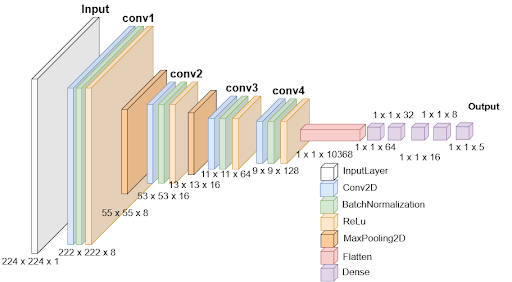
\includegraphics[scale=0.5]{img/pavicnet.png}
            %\caption{Caption}
            \label{fig:enter-label}
        \end{figure}


    \end{columns}
\end{frame}

%---------------------------------------------------------


%---------------------------------------------------------

\begin{frame}
    \frametitle{Problema}
    %\begin{columns}

    %\column{0.5\textwidth}
    \centering
    Doenças e pragas nas folhas do Café Brasileiro mesmo com safra podada (Julho de 2023).


    \begin{figure}
        \centering
        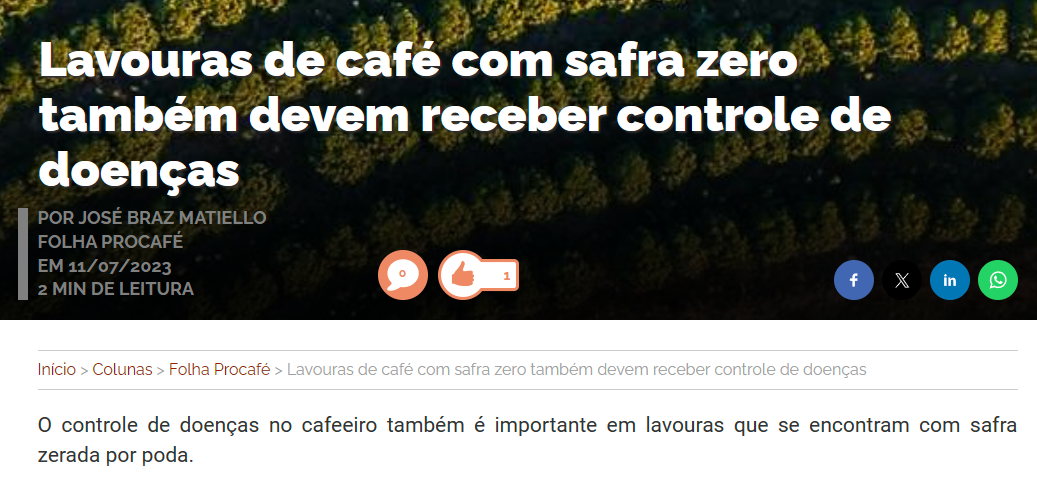
\includegraphics[scale=0.55]{img/safrazero.png}
        \footnote{ \tiny fonte: https://www.cafepoint.com.br/colunas/folha-procafe-jose-braz-matiello/}
        \label{fig:enter-label}
    \end{figure}


\end{frame}

%---------------------------------------------------------


%---------------------------------------------------------

\section{Revisão Bibliográfica} %------------------------------------------------------------------------

\begin{frame}
    \frametitle{Revisão Bibliográfica}
    \begin{columns}

        \column{0.5\textwidth}
        Pequena revisão bibliográfica sobre conceitos abordados neste trabalho:

        \begin{enumerate}
            \item Classificação Binária
            \item Classificação Multiclasse
        \end{enumerate}


        \column{0.5\textwidth}

        \begin{figure}
            \centering
            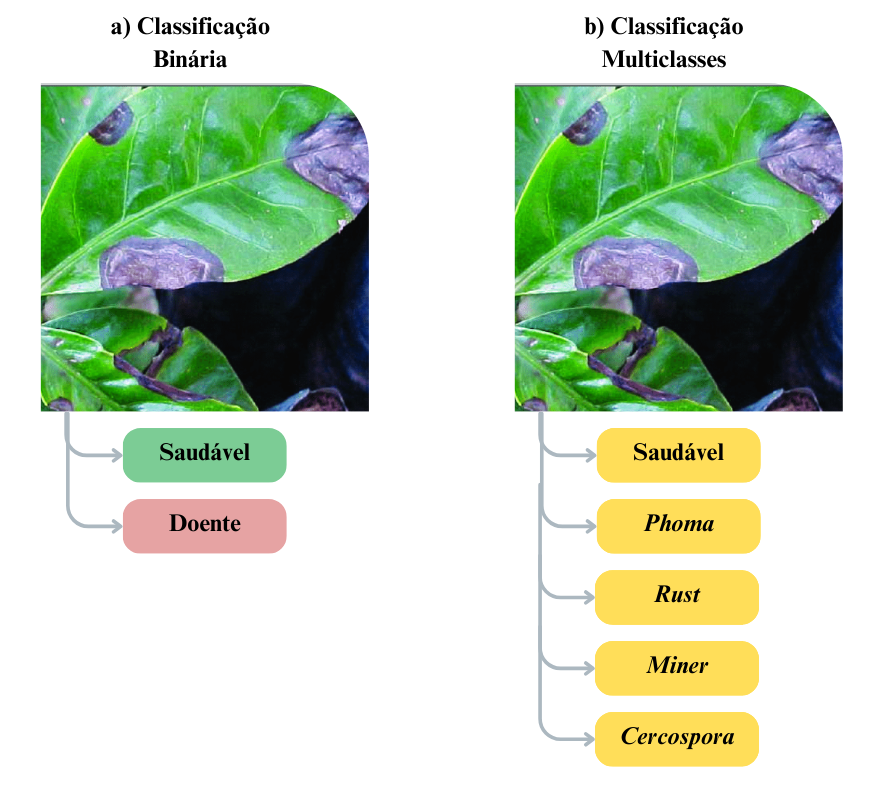
\includegraphics[scale = 0.3 ]{img/ClassificacaoX2 (1).png}
            \label{fig:enter-label}
        \end{figure}


    \end{columns}
\end{frame}

%---------------------------------------------------------



\begin{frame}
    \frametitle{Classificação}
    \begin{columns}
        \column{1\textwidth}

        Classificação Binária ou simplesmente Classificação tem o objetivo de atribuir uma instância a uma de duas classes mutuamente exclusivas.

        \begin{figure}
            \centering
            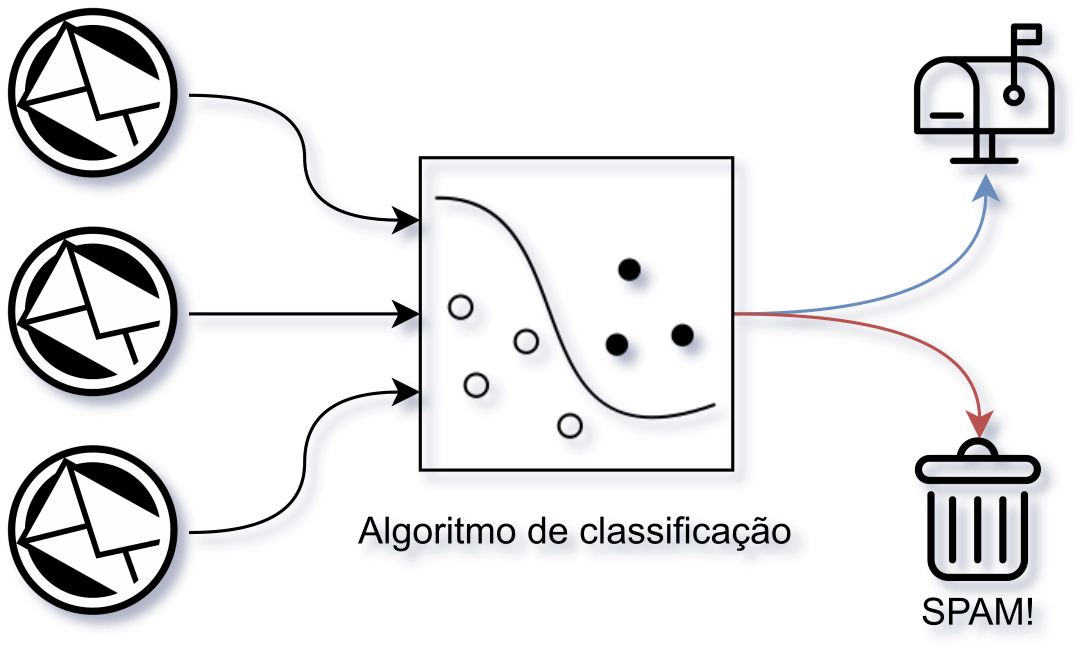
\includegraphics[scale = 0.75 ]{img/email_classifier.png}
            \label{fig:enter-label}
        \end{figure}


    \end{columns}
\end{frame}

%---------------------------------------------------------

%---------------------------------------------------------





\begin{frame}
    \frametitle{Classificação Multiclasse}
    \begin{columns}
        \column{1\textwidth}

        A classificação multilabel lida com problemas em que uma instância pode pertencer a várias classes simultaneamente.

        \begin{figure}
            \centering
            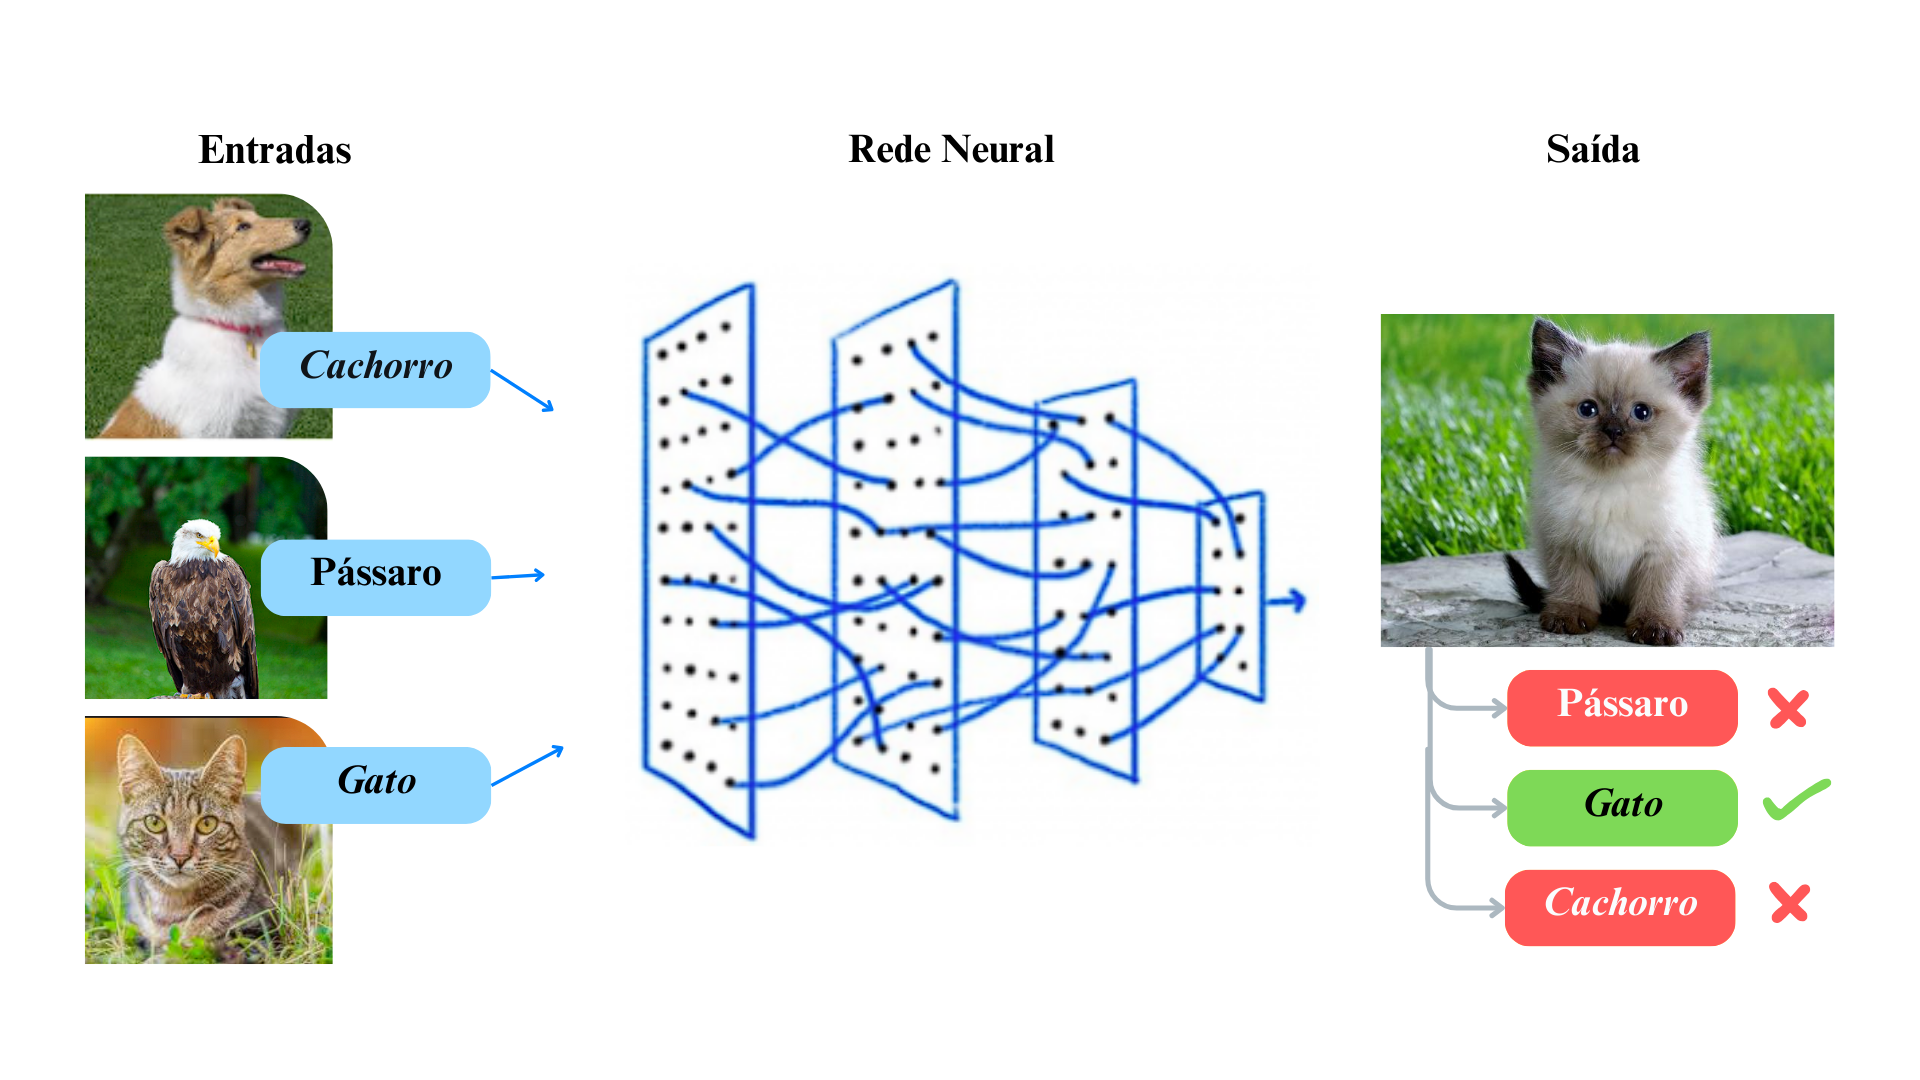
\includegraphics[scale = 0.2 ]{img/multiclassel.png}
            \label{fig:enter-label}
        \end{figure}


    \end{columns}
\end{frame}




%---------------------------------------------------------
\section{Objetivo} %==========================================================================================================


\begin{frame}
    \frametitle{Objetivo}
    \begin{columns}

        \column{0.5\textwidth}

        \begin{itemize}
            \item Classificação automática de doenças e pragas em folhas de café propondo uma arquitetura de classificação eficaz e de baixo custo computacional.
        \end{itemize}


        \column{0.5\textwidth}

        \begin{figure}
            \centering
            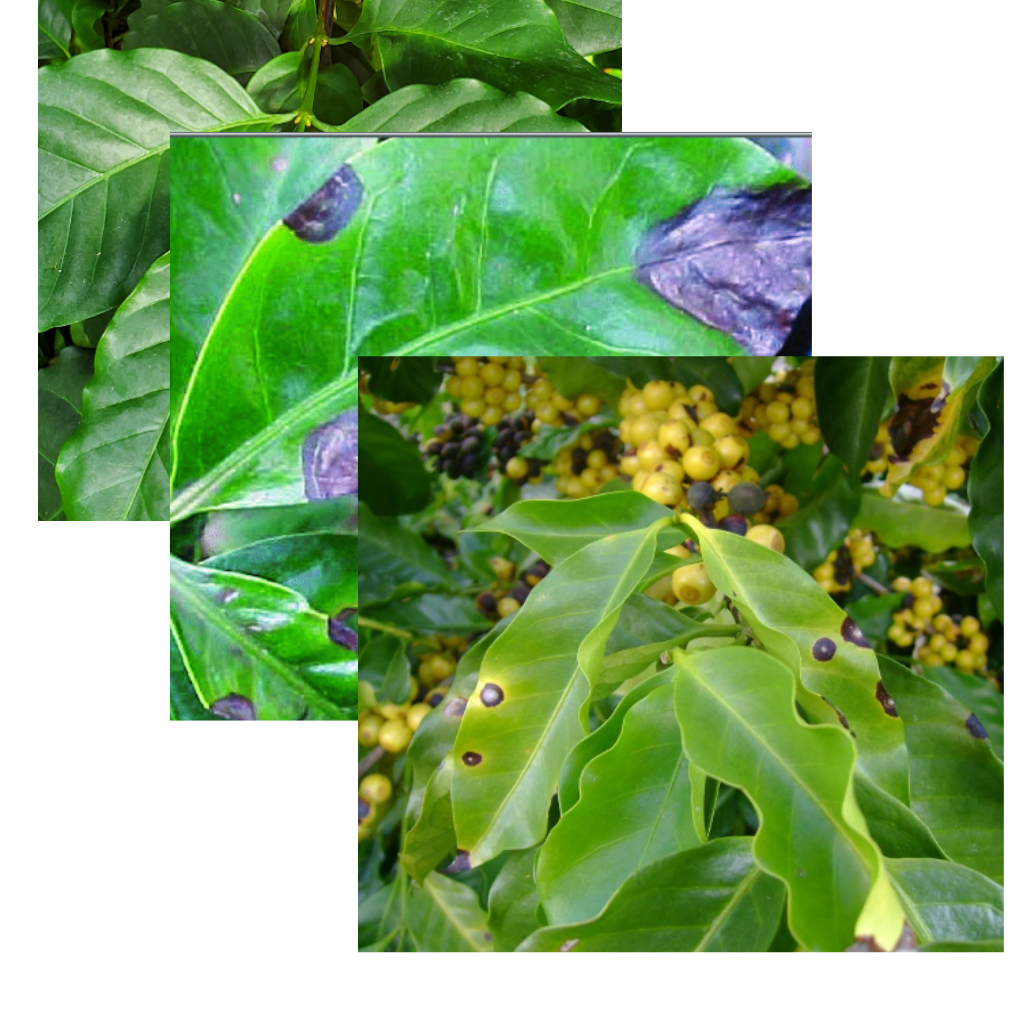
\includegraphics[scale= 0.25]{img/folhass.png}
            %\caption{Caption}
            \label{fig:enter-label}
        \end{figure}

    \end{columns}
\end{frame}

%---------------------------------------------------------


\begin{frame}
    \frametitle{Objetivo}
    \begin{columns}

        \column{0.6\textwidth}

        \begin{itemize}
            \item Realizar o pré-processamento dos datasets JMuBEN, BRACOL, RoCoLe e DiseasesInCoffeeLeaf.
            \item Adaptar a arquitetura PavicNet-MC para otimizar sua eficácia na classificação de doenças e pragas em folhas de café.
            \item Ajustar e configurar os modelos ShuffleNet, ResNet50, InceptionResNetV2, MobileNet V2 e DenseNet169.
            \item Treinar os modelos e avalia-los para classificar em 5 classes: Phoma, Rust, Miner, Cercospora e Healthy.
            \item Comparar o desempenho dos modelos adaptados com o modelo PavicNet-MC.
        \end{itemize}


        \column{0.4\textwidth}
        \vspace{-20px}
        \begin{figure}
            \centering
            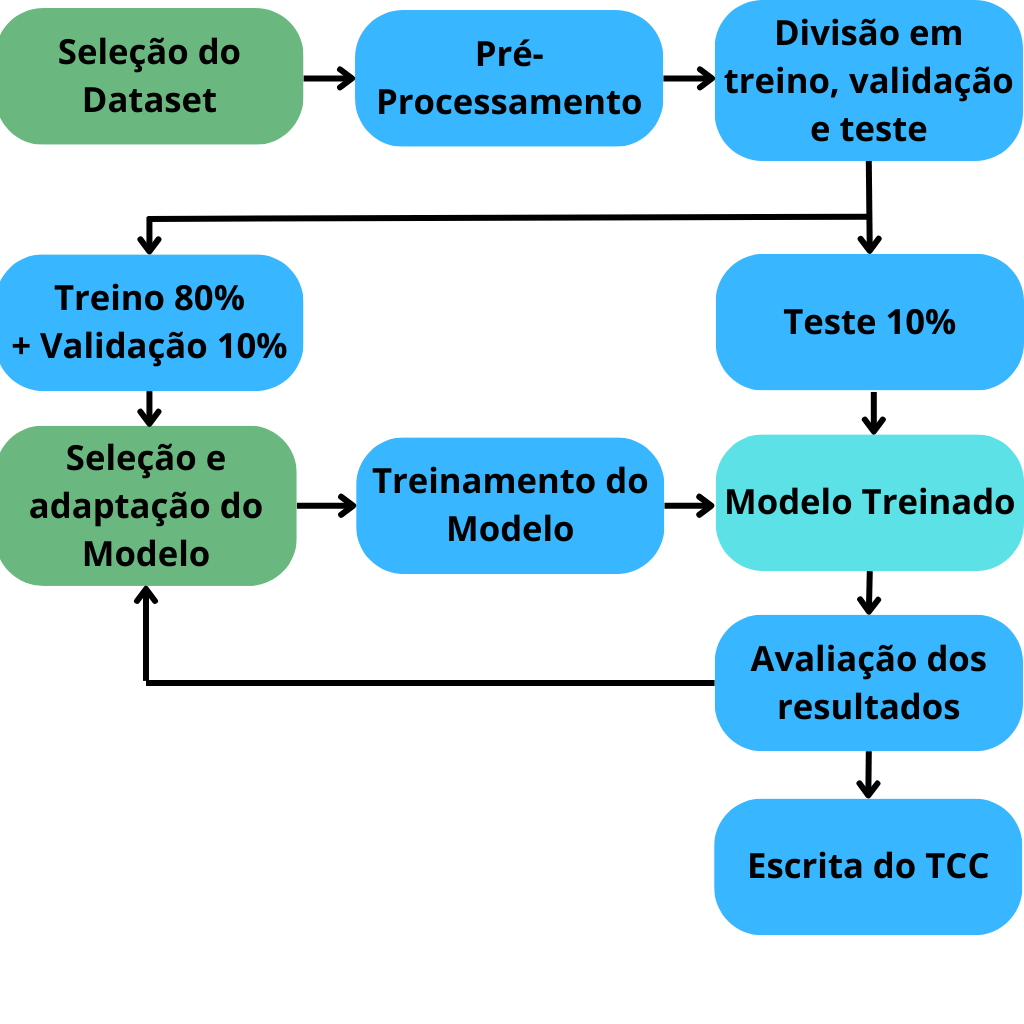
\includegraphics[scale = 0.2]{img/diagrama (2).png}
            \label{fig:enter-label}
        \end{figure}

    \end{columns}
\end{frame}

%---------------------------------------------------------

%---------------------------------------------------------


\begin{frame}
    \frametitle{Dataset (JMuBEN)}


    \begin{figure}
        \centering
        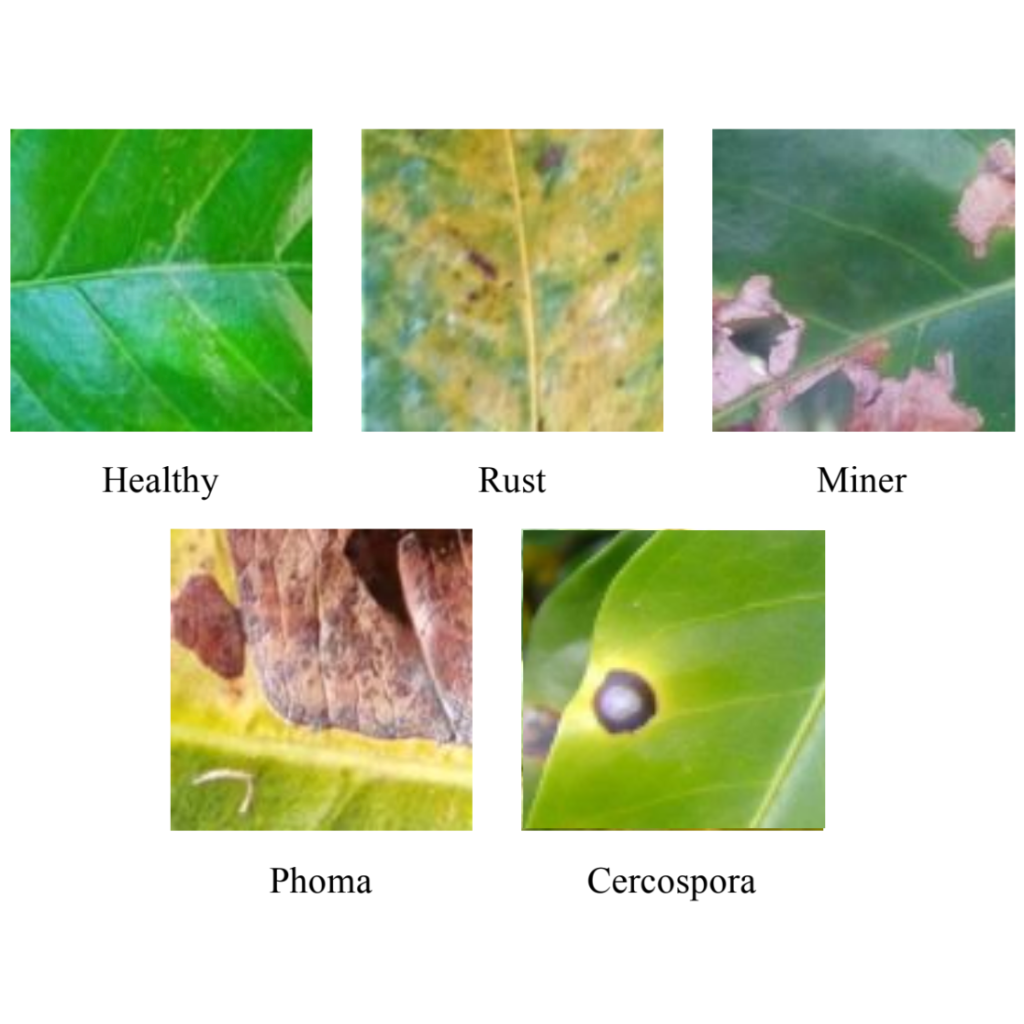
\includegraphics[scale = 0.3]{img/classes.png}
        %\caption{Caption}
        \label{fig:enter-label}
    \end{figure}

\end{frame}

%---------------------------------------------------------



%---------------------------------------------------------


\begin{frame}
    \frametitle{Dataset (BRACOL)}
    \centering
    Healthy, Cercospora, Miner, Rust and Phoma.
    \begin{figure}
        \centering
        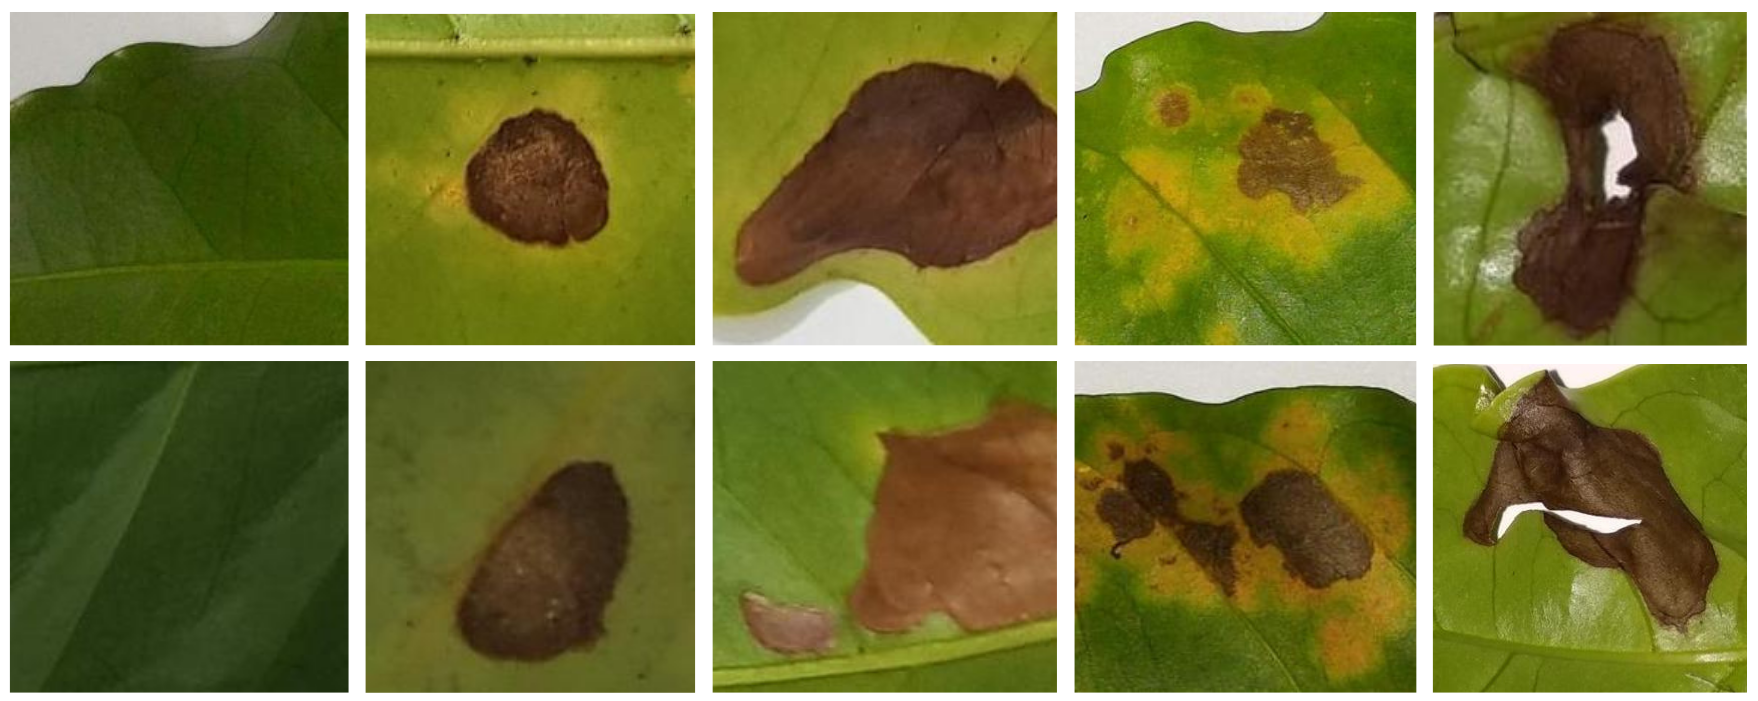
\includegraphics[scale = 0.27]{img/SintomDatasetExample.png}
        %\caption{Caption}
        \label{fig:enter-label}
    \end{figure}

\end{frame}

%---------------------------------------------------------



%---------------------------------------------------------


\begin{frame}
    \frametitle{Dataset (RoCole e Disease and pest in coffee leaves)}

    \centering
    Rust and Red Spider Mite.
    \begin{figure}
        \centering
        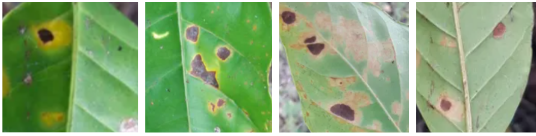
\includegraphics[scale = 0.9]{img/RocoleExample.png}
        %\caption{Caption}
        \label{fig:enter-label}
    \end{figure}

    \centering
    Miner and Rust
    \begin{figure}
        \centering
        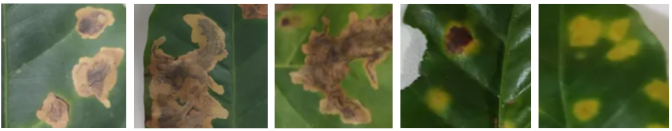
\includegraphics[scale = 0.8]{img/DesiaseandpestExemple.png}
        %\caption{Caption}
        \label{fig:enter-label}
    \end{figure}


\end{frame}

%---------------------------------------------------------



%---------------------------------------------------------
\section{Metodologia}


\begin{frame}
    \frametitle{Metodologia}
    \begin{columns}

        \column{0.5\textwidth}

        \begin{itemize}
            \item Hardware e Software:
                  \begin{itemize}
                      \item Python (Keras e Tensorflow)
                      \item Google Colab
                  \end{itemize}
            \item Métricas de Avaliação:
                  \begin{itemize}
                      \item Matriz de Confusão
                      \item Acurácia
                      \item Precisão
                      \item Área sobre a curva ROC
                  \end{itemize}
                  % \item Arquiteturas:
                  % \begin{itemize}
                  %     \item PavicNet-MC
                  %     \item ResNet50
                  %     \item InceptionResNetV2
                  %     \item MobileNet V2
                  %     \item DenseNet169
                  % \end{itemize}
            \item Dataset (JMuBEN, BRACOL, RoCoLe e DPCL)
        \end{itemize}

        \column{0.5\textwidth}

        \begin{figure}
            \centering
            
\includegraphics[scale = 0.2]{img/python_colab.png}
            \label{fig:enter-label}
        \end{figure}

    \end{columns}
\end{frame}

%---------------------------------------------------------


%---------------------------------------------------------

\section{Referência}

\begin{frame}
    \frametitle{Referência}

    \begin{block}{}
        Web-based CNN Application for Arabica Coffee Leaf Disease Prediction in Smart Agriculture
    \end{block}

    \begin{figure}
        \centering
        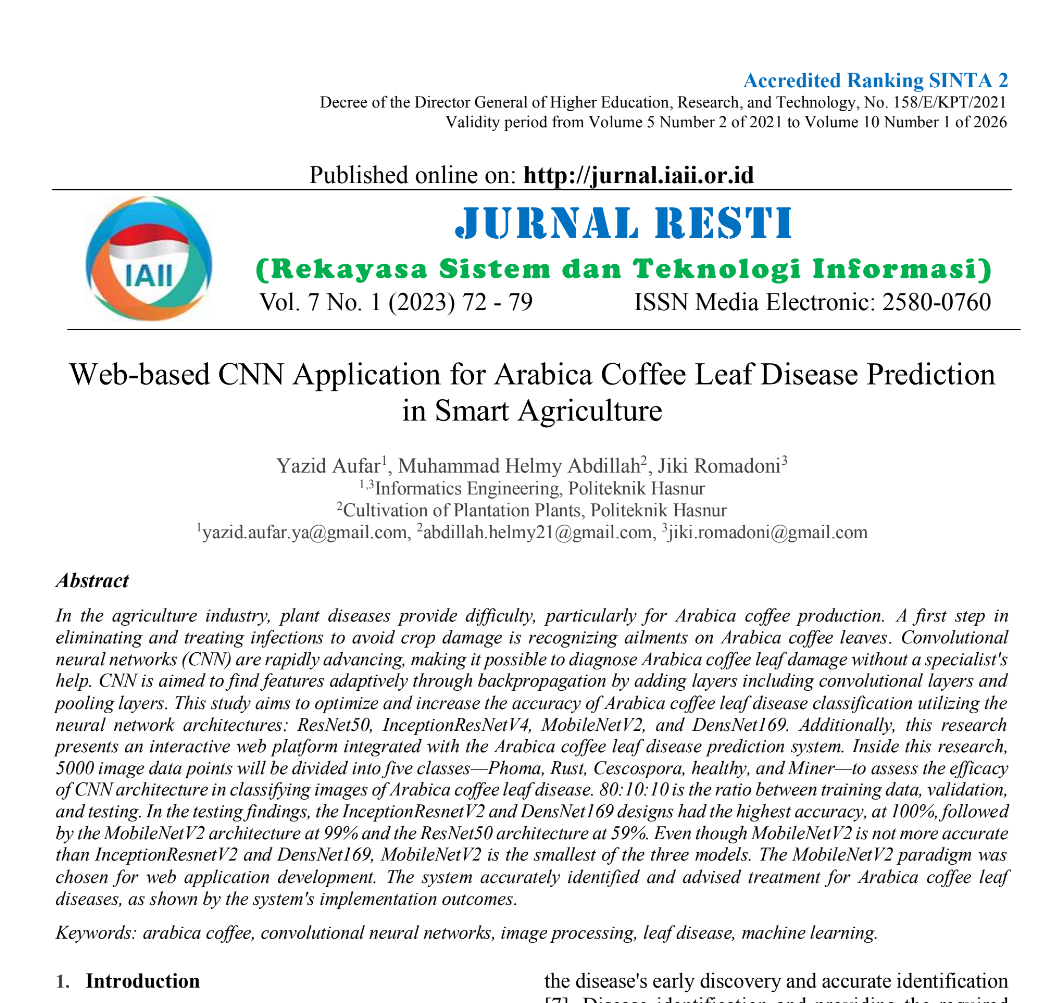
\includegraphics[scale = 0.35 ]{img/ref.png}
        \label{fig:enter-label}
    \end{figure}

\end{frame}


% --------------------------------------------------------------------------------------------------


\begin{frame}
    \frametitle{Próximos Passos}

    \begin{block}{Curto Prazo:}

        Replicar o trabalho do artigo de referência:
        \begin{itemize}
            \item Implementar as 4 arquiteturas restantes
            \item Iniciar o treinamento e validação dessas arquiteturas
        \end{itemize}

    \end{block}



    \begin{block}{Médio Prazo:}

        \begin{itemize}
            \item Dar continuidade a escrita do TCC
        \end{itemize}

    \end{block}




\end{frame}


%---------------------------------------------------------
\section{Avanços 10/11}


\begin{frame}
    \frametitle{Avanços: 10 de Outubro}
    \begin{columns}


        \column{0.5\textwidth}

        Implementado as arquiteturas do artigo de referência:

        \begin{itemize}
            \item Resnet50
            \item InceptionResnetV2
            \item MobilenetV2
            \item DenseNet169
        \end{itemize}

        \column{0.5\textwidth}

        \begin{itemize}
            \item Balanceamento do dataset com base no artigo base
        \end{itemize}


    \end{columns}

\end{frame}

%---------------------------------------------------------


%---------------------------------------------------------



\begin{frame}
    \frametitle{Resultados preliminares}

    \centering


    \begin{columns}


        \column{0.5\textwidth}

        \centering
        Dataset JMUBEN original
        \begin{figure}
            \centering
            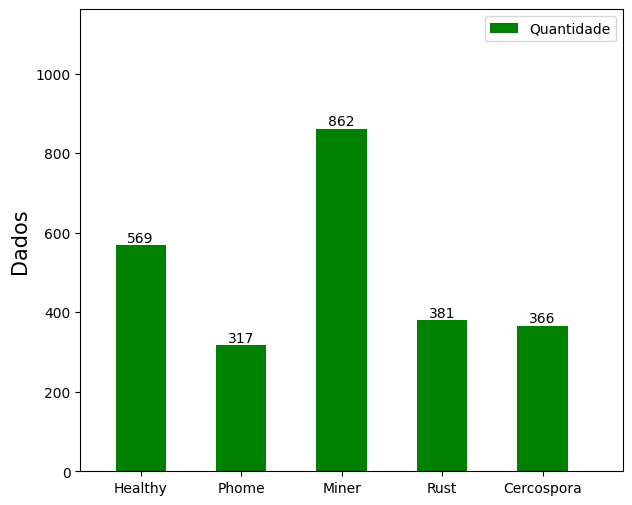
\includegraphics[scale=0.39]{img/jmubennormal.png}
            %\caption{Res}
            \label{fig:enter-label}
        \end{figure}
        \centering


        \column{0.5\textwidth}

        \centering
        Dataset JMUBEN original com data augumentation e balanceamento
        \begin{figure}
            \centering
            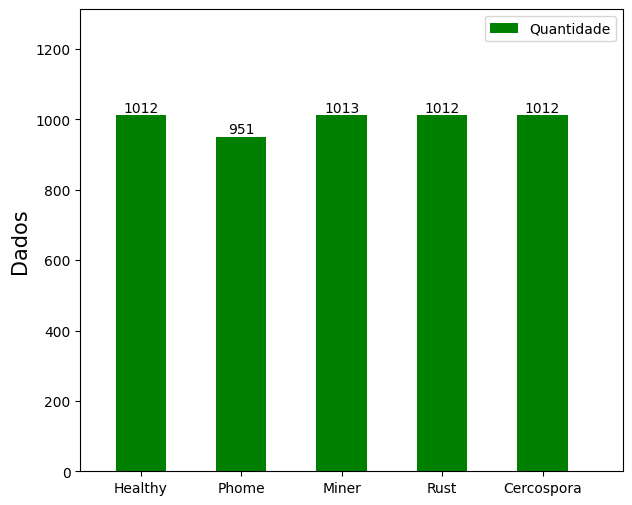
\includegraphics[scale=0.39]{img/jmubenbalanceado.png}
            %\caption{Res}
            \label{fig:enter-label}
        \end{figure}



    \end{columns}
\end{frame}

%---------------------------------------------------------


%---------------------------------------------------------



\begin{frame}
    \frametitle{Resultados Preliminares}

    \centering
    Resultados preliminares:

    \begin{columns}


        \column{0.5\textwidth}

        \centering
        \tiny Modelo: PavicNet-MC
        \begin{figure}
            \centering
            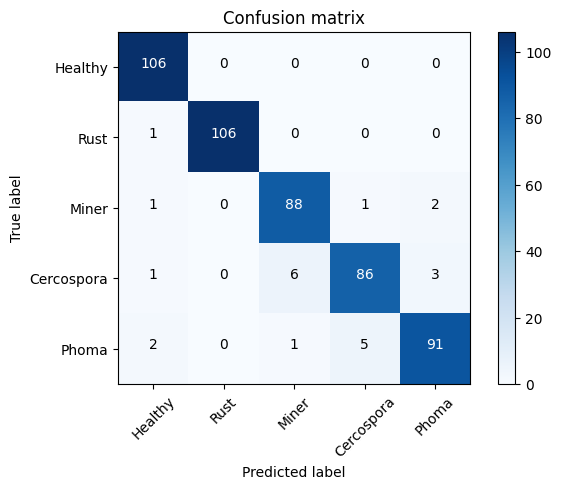
\includegraphics[scale=0.39]{img/Pavicnetresult1.png}
            %\caption{Res}
            \label{fig:enter-label}
        \end{figure}
        \centering


        \column{0.5\textwidth}

        \centering
        \tiny Modelo: InceptionResnetV2
        \begin{figure}
            \centering
            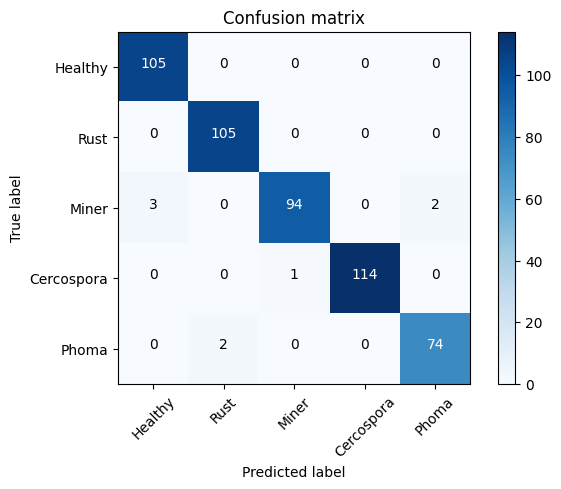
\includegraphics[scale=0.39]{img/Inceptionresult1.png}
            %\caption{Res}
            \label{fig:enter-label}
        \end{figure}



    \end{columns}
\end{frame}

%---------------------------------------------------------



\begin{frame}
    \frametitle{Resultados Preliminares}



    \centering
    \tiny Modelo: Resnet50
    \begin{figure}
        \centering
        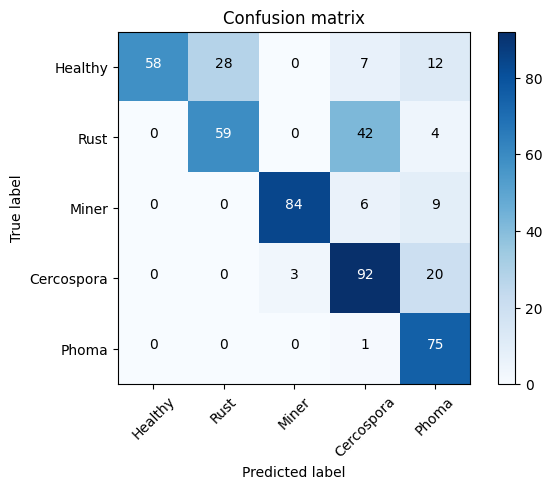
\includegraphics[scale=0.45]{img/resnet50result1.png}
        %\caption{Res}
        \label{fig:enter-label}
    \end{figure}



\end{frame}


%----------------------------------------------------------------------------------


% -------------------------------------------------------------------
\section{Próximos Passos}

\begin{frame}
    \frametitle{Próximos Passos}

    \begin{block}{Curto Prazo:}

        \begin{itemize}
            \item Terminar o treinamento e validação dessas arquiteturas
            \item  Comparar resultados com o artigo de referência
        \end{itemize}

    \end{block}



    \begin{block}{Médio Prazo:}

        \begin{itemize}
            \item Dar continuidade a escrita do TCC
        \end{itemize}

    \end{block}




\end{frame}




% -----------------------------------------------------------------------------------






%---------------------------------------------------------



\begin{frame}
    \frametitle{Resultados Preliminares}

    \centering


    \begin{columns}


        \column{0.5\textwidth}

        \centering
        \tiny Modelo: InceptionResnetV2 Treinada
        \begin{figure}
            \centering
            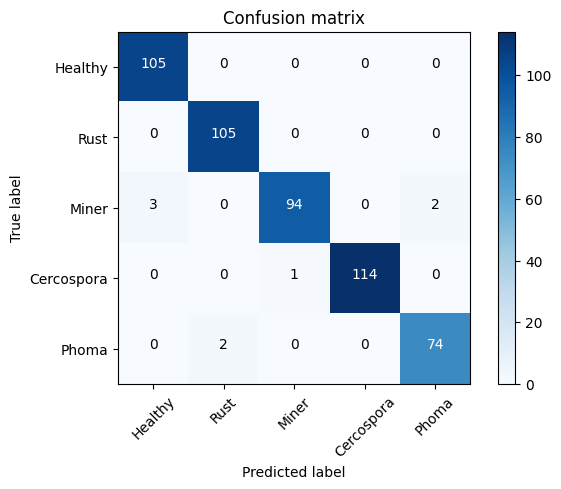
\includegraphics[scale=0.39]{img/Inceptionresult1.png}
            %\caption{Res}
            \label{fig:enter-label}
        \end{figure}
        \centering


        \column{0.5\textwidth}

        \centering
        \tiny Modelo: InceptionResnetV2 de Referência
        \begin{figure}
            \centering
            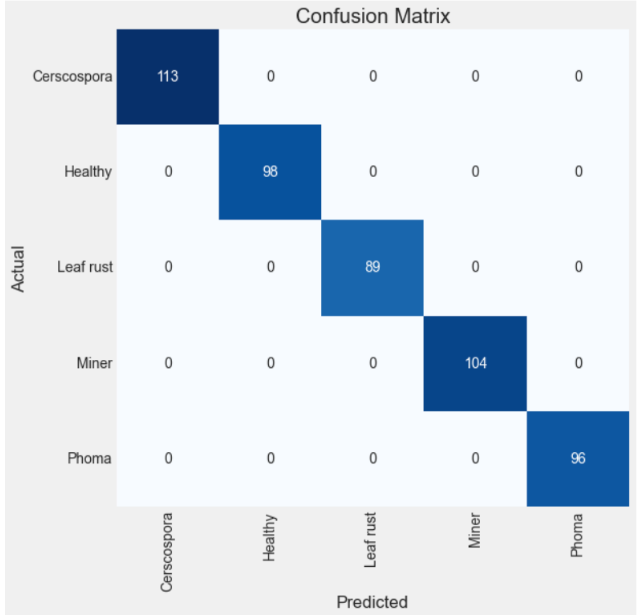
\includegraphics[scale=0.39]{img/inceptionreferencia.png}
            %\caption{Res}
            \label{fig:enter-label}
        \end{figure}



    \end{columns}
\end{frame}

%---------------------------------------------------------

%---------------------------------------------------------



\begin{frame}
    \frametitle{Resultados Preliminares}

    \centering


    \begin{columns}


        \column{0.5\textwidth}

        \centering
        \tiny Modelo: Resnet50 Treinada
        \begin{figure}
            \centering
            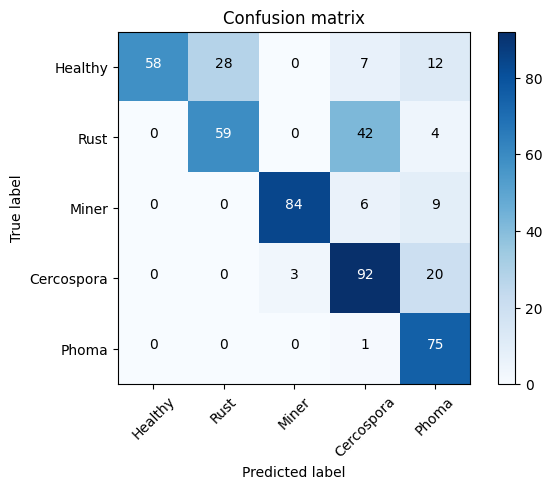
\includegraphics[scale=0.39]{img/resnet50result1.png}
            %\caption{Res}
            \label{fig:enter-label}
        \end{figure}
        \centering


        \column{0.5\textwidth}

        \centering
        \tiny Modelo: Resnet50 de Referência
        \begin{figure}
            \centering
            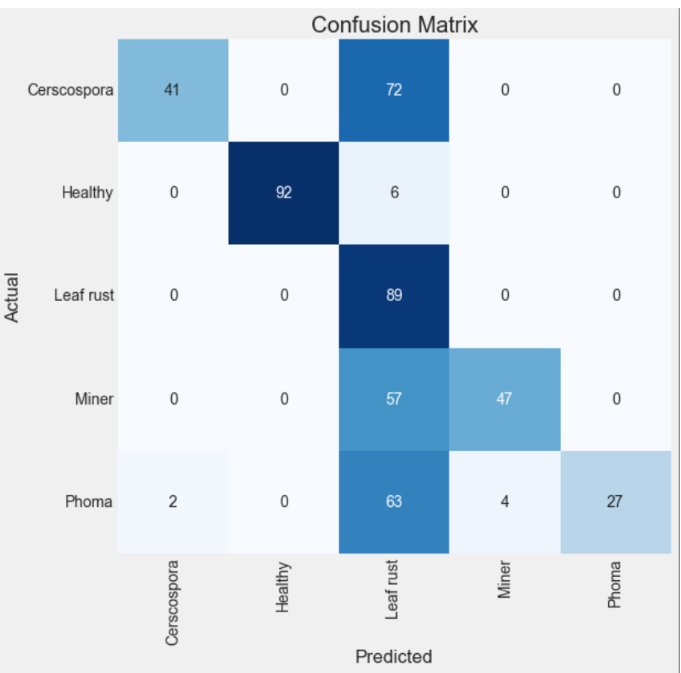
\includegraphics[scale=0.35]{img/resnetdereferencia.png}
            %\caption{Res}
            \label{fig:enter-label}
        \end{figure}



    \end{columns}
\end{frame}

%---------------------------------------------------------


%---------------------------------------------------------



\begin{frame}
    \frametitle{Resultados Preliminares}

    \centering


    \begin{columns}


        \column{0.5\textwidth}

        \centering
        \tiny Modelo: MobileNetV2 Treinada
        \begin{figure}
            \centering
            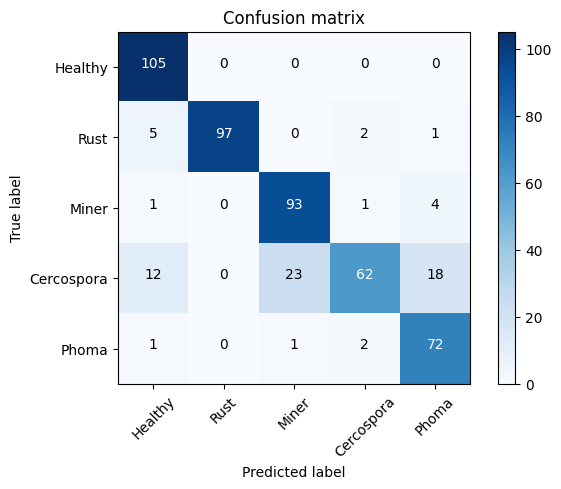
\includegraphics[scale=0.39]{img/MobilenetResult1.png}
            %\caption{Res}
            \label{fig:enter-label}
        \end{figure}
        \centering


        \column{0.5\textwidth}

        \centering
        \tiny Modelo: MobileNetV2 de Referência
        \begin{figure}
            \centering
            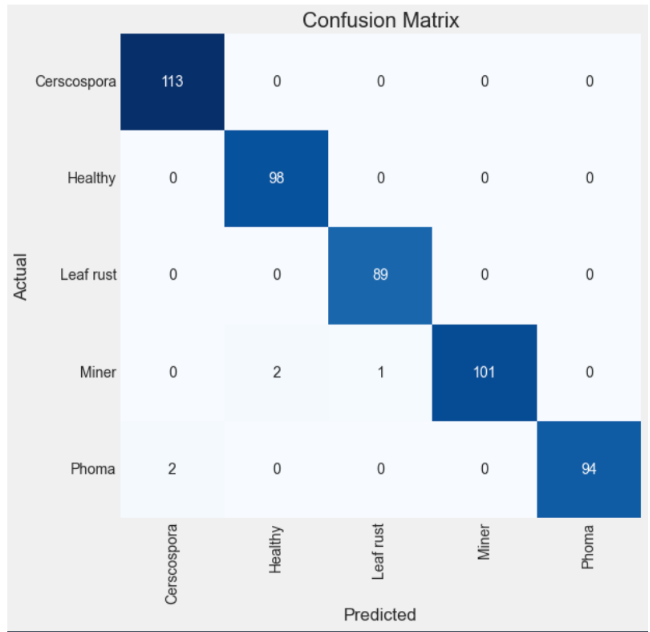
\includegraphics[scale=0.35]{img/mobilenetreferencia.png}
            %\caption{Res}
            \label{fig:enter-label}
        \end{figure}



    \end{columns}
\end{frame}

%---------------------------------------------------------



%---------------------------------------------------------



\begin{frame}
    \frametitle{Resultados Preliminares}

    \centering


    \begin{columns}


        \column{0.5\textwidth}

        \centering
        \tiny Modelo: Densenet169 Treinada
        \begin{figure}
            \centering
            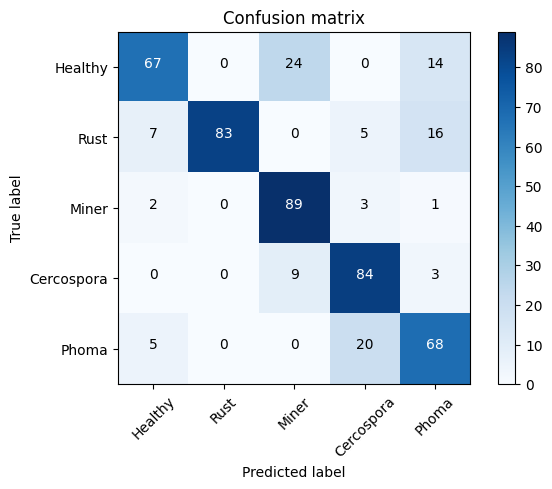
\includegraphics[scale=0.39]{img/densenet169result1.png}
            %\caption{Res}
            \label{fig:enter-label}
        \end{figure}
        \centering


        \column{0.5\textwidth}

        \centering
        \tiny Modelo: Densenet169 de Referência
        \begin{figure}
            \centering
            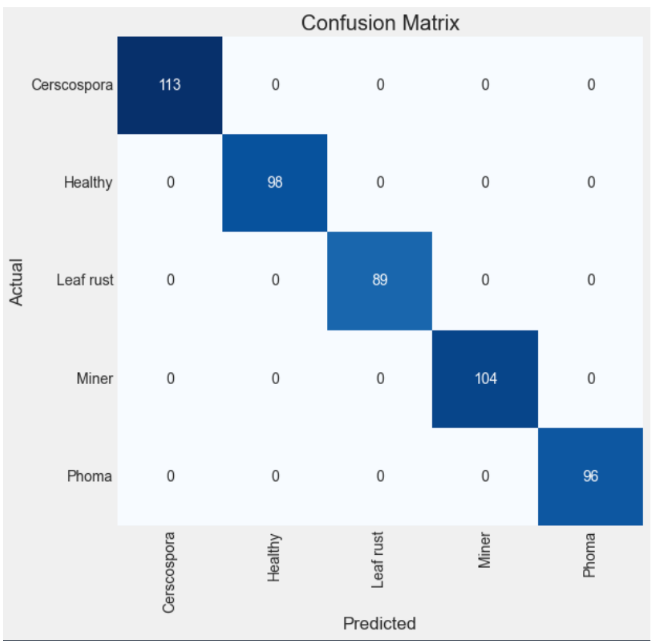
\includegraphics[scale=0.35]{img/densenet169referencia.png}
            %\caption{Res}
            \label{fig:enter-label}
        \end{figure}



    \end{columns}
\end{frame}

%---------------------------------------------------------





%---------------------------------------------------------



\begin{frame}
    \frametitle{Resultados Preliminares}

    \centering


    \begin{columns}


        \column{0.5\textwidth}

        \centering
        \tiny Modelo: PavicNet-MC Treinada
        \begin{figure}
            \centering
            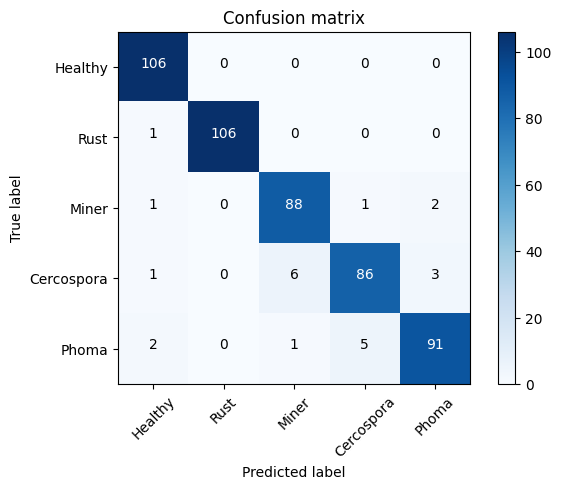
\includegraphics[scale=0.5]{img/Pavicnetresult1.png}
            %\caption{Res}
            \label{fig:enter-label}
        \end{figure}
        \centering

        \column{0.5\textwidth}
        Accuracy for Healthy: 1.0 \footnote{Classe com problemas}

        Accuracy for leaf rust: 0.998 \footnote{Classe com problemas}

        Accuracy for miner: 0.978

        Accuracy for cercospora: 0.968

        Accuracy for phoma: 0.974




    \end{columns}
\end{frame}

%---------------------------------------------------------











\begin{frame}
    \frametitle{Resultados Preliminares}

    \centering


    \begin{columns}


        \column{0.5\textwidth}

        \centering
        \tiny Modelo: Densenet169
        \begin{figure}
            \centering
            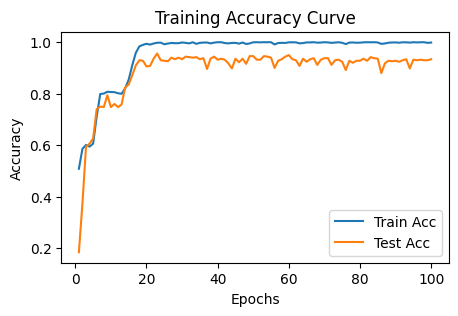
\includegraphics[scale=0.5]{img/Notebook_57_1.png}
            %\caption{Res}
            \label{fig:enter-label}
        \end{figure}
        \centering


        \column{0.5\textwidth}

        \centering
        \begin{figure}
            \centering
            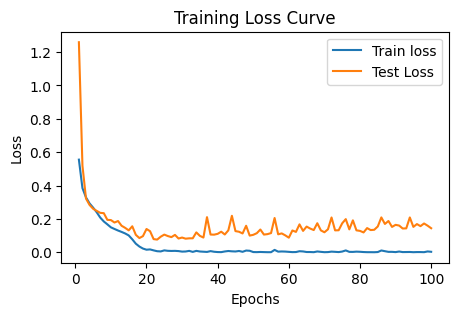
\includegraphics[scale=0.5]{img/Notebook_57_0.png}
            %\caption{Res}
            \label{fig:enter-label}
        \end{figure}



    \end{columns}
\end{frame}





% ----------------------------------------------------------------------------------------------------------------------------




\section{Próximos Passos}

\begin{frame}
    \frametitle{Próximos Passos}

    \begin{block}{Curto Prazo:}

        \begin{itemize}
            \item Pesquisar e definir novos datasets
            \item Treinar os modelos implementados com os novos datasets
        \end{itemize}

    \end{block}



    \begin{block}{Médio Prazo:}

        \begin{itemize}
            \item Apresentação do artigo no Healthinf
            \item Dar continuidade a escrita do TCC
        \end{itemize}

    \end{block}




\end{frame}


%---------------------------------------------------------

\begin{frame}
    \frametitle{Próximos Passos}

    \begin{block}{Curto Prazo:}

        \begin{itemize}
            \item Pesquisar e definir novos datasets. \textsc{Concluído}
            \item Pré-Processar os novos datasets. \textsc{Concluído}
            \item Treinar os modelos implementados com os novos datasets.
        \end{itemize}

    \end{block}



    \begin{block}{Médio Prazo:}

        \begin{itemize}
            \item Apresentação do artigo no Healthinf. \textsc{Concluído}
            \item Dar continuidade a escrita do TCC.
        \end{itemize}

    \end{block}




\end{frame}

% -----------------------------------------------------------------------



\begin{frame}
    \frametitle{Resultados preliminares}


    \centering
    Dataset BRACOL

    \begin{figure}
        \centering
        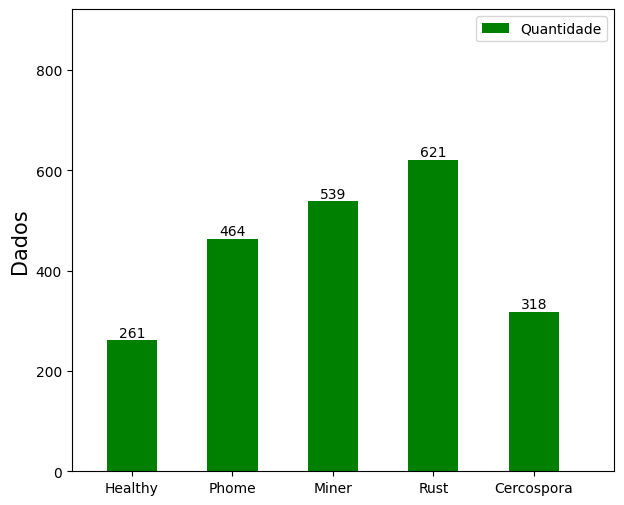
\includegraphics[scale = 0.5]{img/bracol data.png}
        %\caption{Caption}
        \label{fig:enter-label}
    \end{figure}

\end{frame}

% %---------------------------------------------------------



\begin{frame}
    \frametitle{Resultados preliminares}


    \centering
    Dataset BRACOL

    \begin{figure}
        \centering
        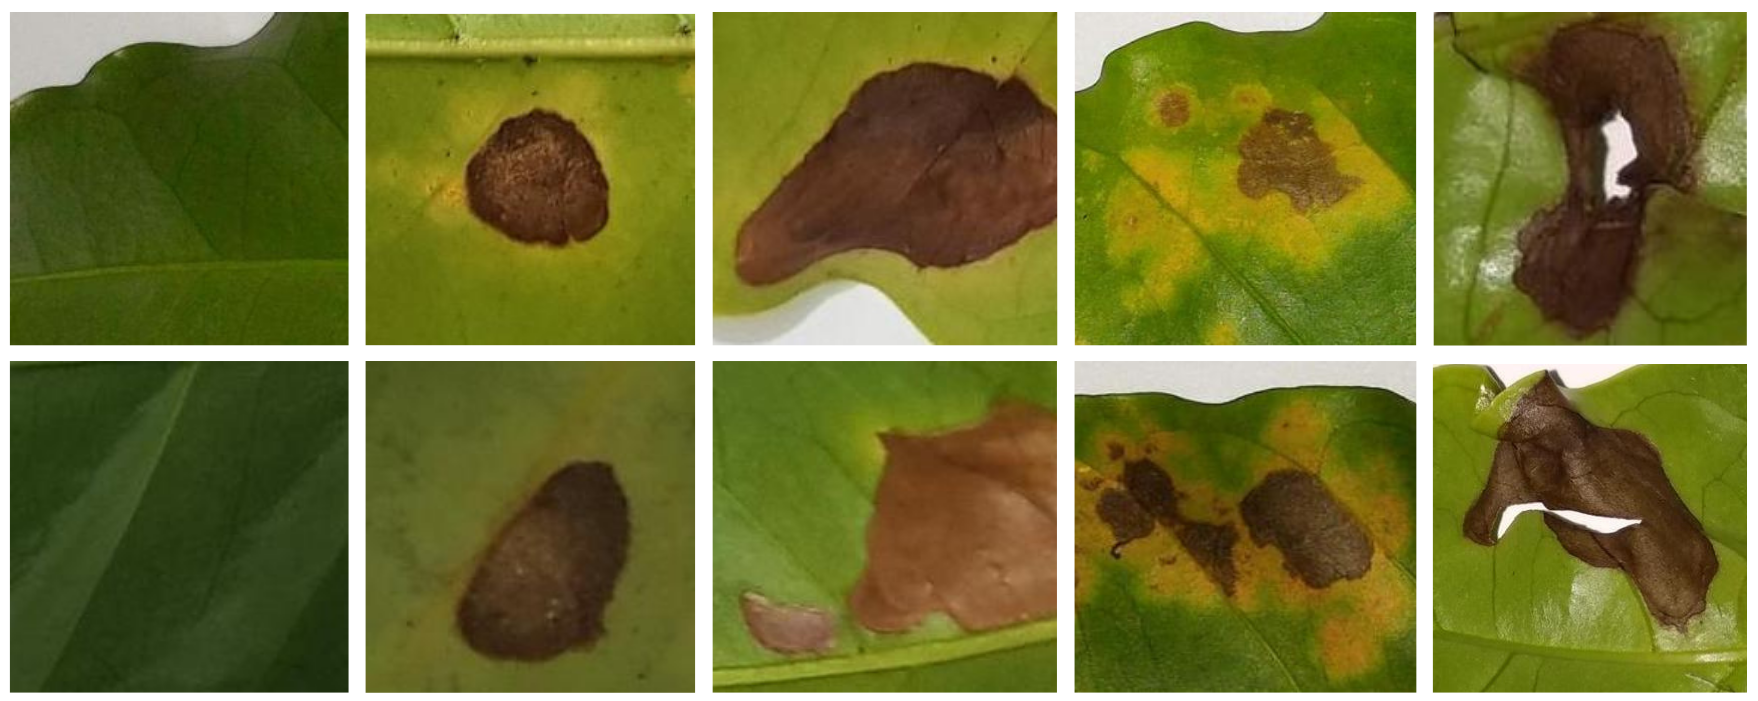
\includegraphics[scale = 0.27]{img/SintomDatasetExample.png}
        %\caption{Caption}
        \label{fig:enter-label}
    \end{figure}

\end{frame}



% %=======================================================================
% \begin{frame}
%     \frametitle{Resultados preliminares}


%     \begin{columns}


%         \column{0.5\textwidth}

%         \centering
%         PavicNet-MC GrayScale

%         \begin{figure}
%             \centering
%             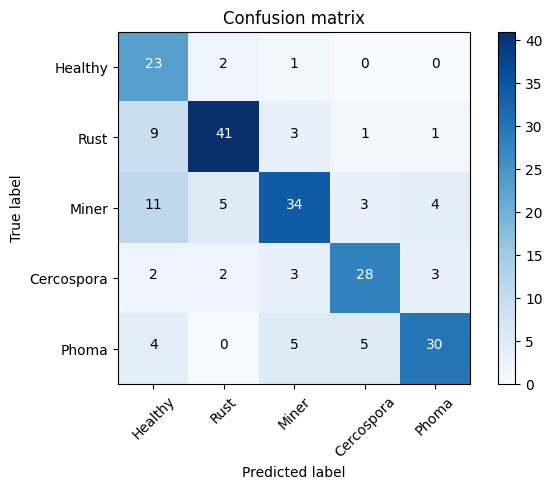
\includegraphics[scale = 0.5]{img/MatrizPavicNetBracolGray.png}
%             %\caption{Caption}
%             \label{fig:enter-label}
%         \end{figure}


%         \column{0.5\textwidth}

%         The accuracy for Healthy: 0.9636

%         The accuracy for leaf_rust: 0.8954

%         The accuracy for miner: 0.8363

%         The accuracy for cerscospora: 0.9136

%         The accuracy for phoma: 0.9045



%     \end{columns}
% \end{frame}



% %---------------------------------------------------------



% \begin{frame}
%     \frametitle{Resultados preliminares}


%     \begin{columns}


%         \column{0.5\textwidth}

%         \centering
%         PavicNet-MC RGB

%         \begin{figure}
%             \centering
%             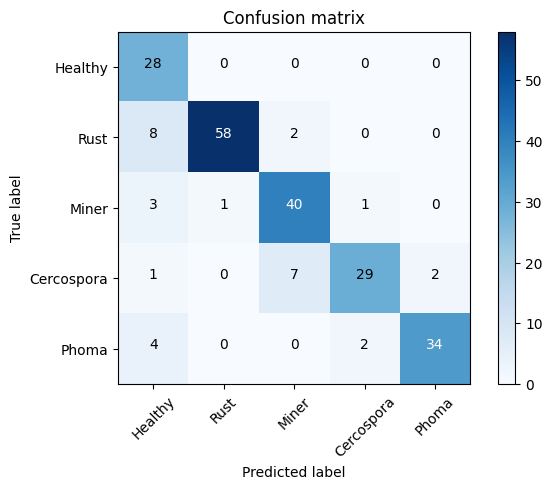
\includegraphics[scale = 0.5]{img/pavicNetBracolRGB.png}
%             %\caption{Caption}
%             \label{fig:enter-label}
%         \end{figure}


%         \column{0.5\textwidth}


%         The accuracy for Healthy: 0.9727

%         The accuracy for leaf_rust: 0.95

%         The accuracy for miner: 0.9363

%         The accuracy for cerscospora: 0.9409

%         The accuracy for phoma: 0.9636



%     \end{columns}
% \end{frame}




% %---------------------------------------------------------

\begin{frame}
    \frametitle{Resultados preliminares}


    \centering
    Curvas de treinamento

    \begin{columns}

        \column{0.5\textwidth}


        \begin{figure}
            \centering
            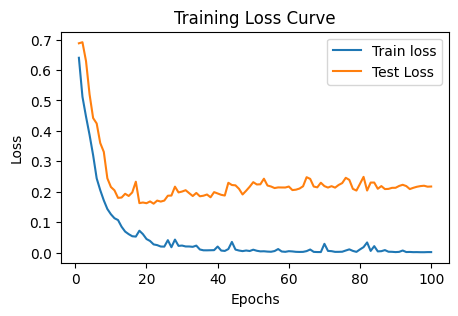
\includegraphics[scale = 0.6]{img/lossbracol.png}
            %\caption{Caption}
            \label{fig:enter-label}
        \end{figure}


        \column{0.5\textwidth}


        \begin{figure}
            \centering
            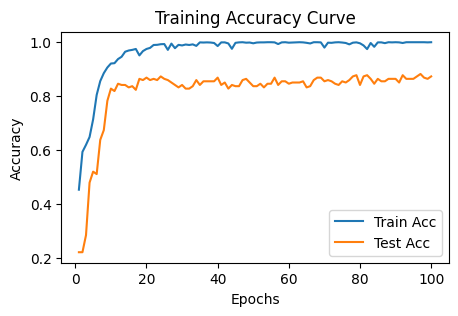
\includegraphics[scale = 0.6]{img/accbracol.png}
            %\caption{Caption}
            \label{fig:enter-label}
        \end{figure}


    \end{columns}
\end{frame}


% %---------------------------------------------------------



\begin{frame}
    \frametitle{Resultados preliminares}


    \centering

    \begin{figure}
        \centering
        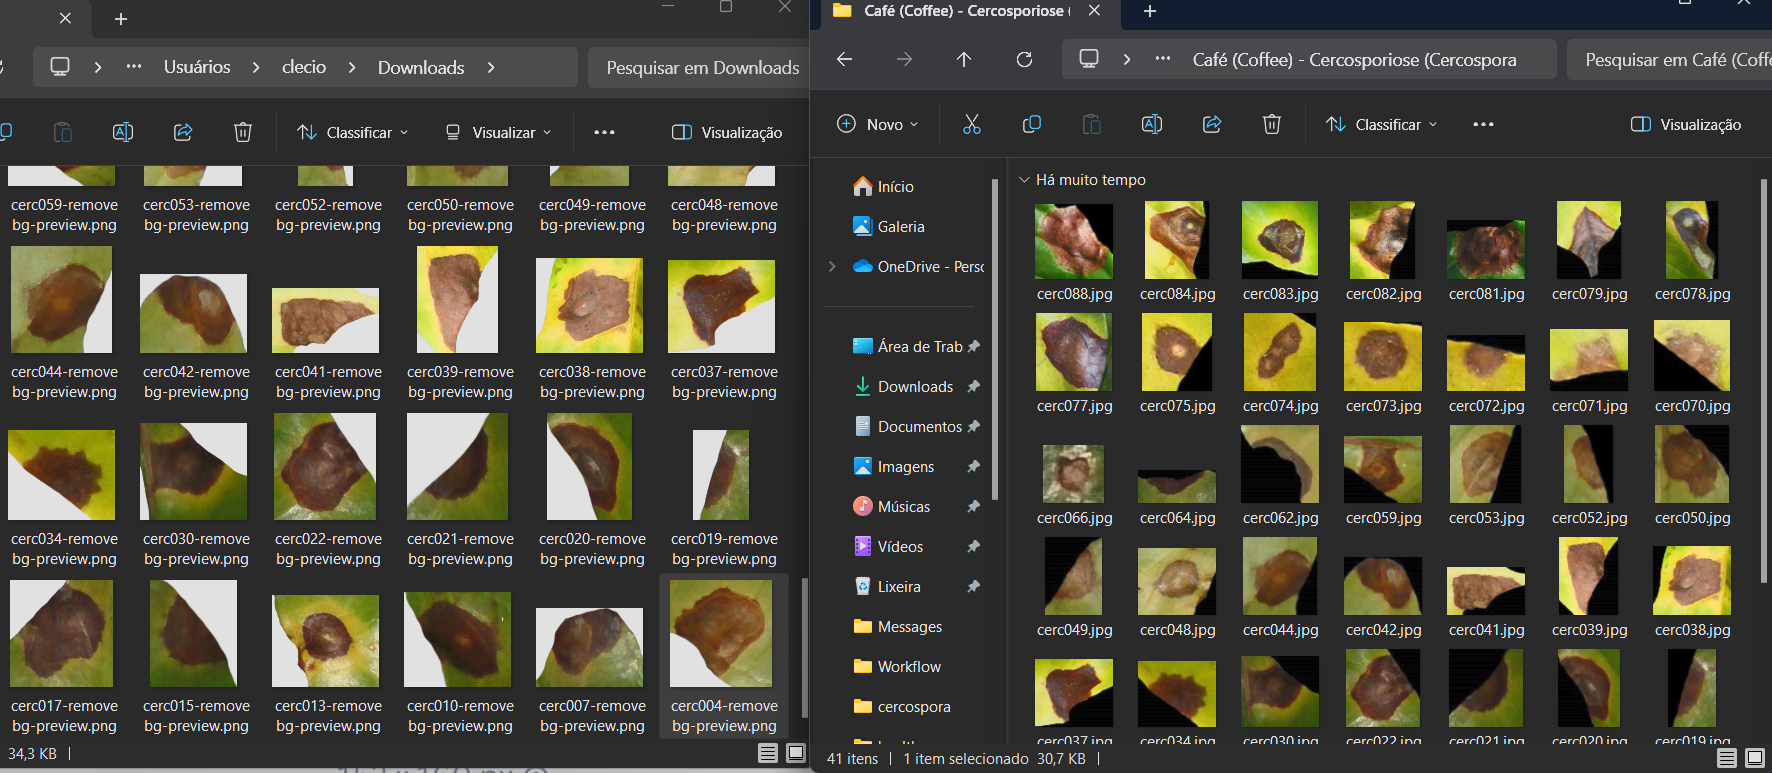
\includegraphics[scale = 0.45]{img/Captura de tela 2024-04-03 104343.png}
        %\caption{Caption}
        \label{fig:enter-label}
    \end{figure}

\end{frame}



% %=======================================================================






% -----------------------------------------------------------------------



\begin{frame}
    \frametitle{Resultados preliminares}


    \centering
    Dataset BRACOL

    \begin{columns}

        \column{0.5\textwidth}


        \begin{figure}
            \centering
            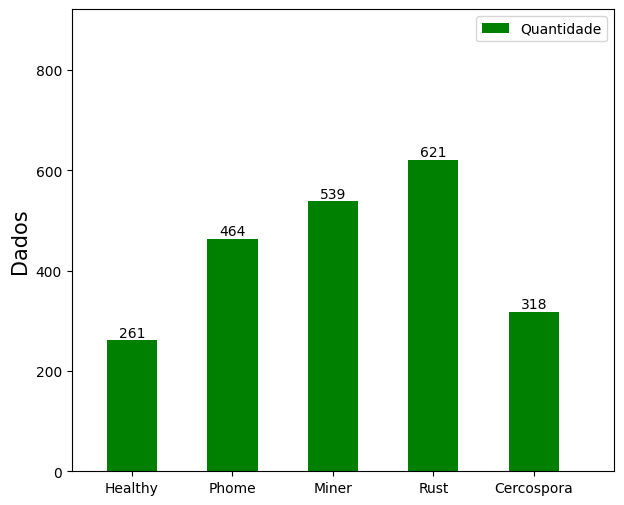
\includegraphics[scale = 0.45]{img/bracol data.png}
            %\caption{Caption}
            \label{fig:enter-label}
        \end{figure}


        \column{0.5\textwidth}


        \begin{figure}
            \centering
            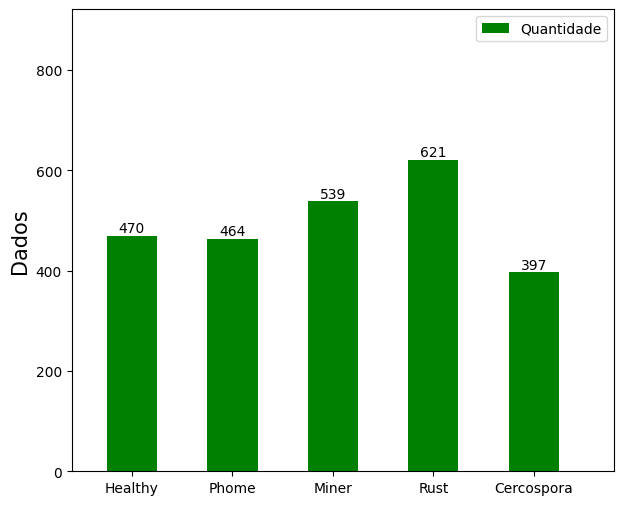
\includegraphics[scale = 0.45]{img/bracoldatabalanced.png}
            %\caption{Caption}
            \label{fig:enter-label}
        \end{figure}


    \end{columns}
\end{frame}

% %---------------------------------------------------------




\begin{frame}
    \frametitle{Resultados preliminares}


    \centering
    Após ajustes

    \begin{columns}

        \column{0.5\textwidth}


        \begin{figure}
            \centering
            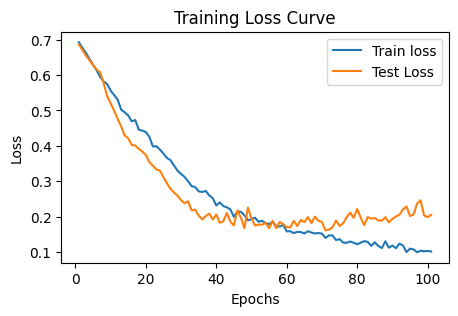
\includegraphics[scale = 0.6]{img/baixados.png}
            %\caption{Caption}
            \label{fig:enter-label}
        \end{figure}


        \column{0.5\textwidth}


        \begin{figure}
            \centering
            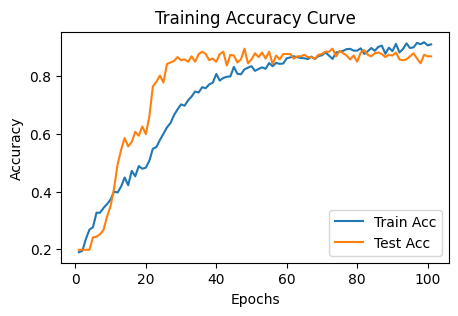
\includegraphics[scale = 0.6]{img/baixados (1).png}
            %\caption{Caption}
            \label{fig:enter-label}
        \end{figure}


    \end{columns}
\end{frame}

% %---------------------------------------------------------


% %---------------------------------------------------------



\begin{frame}
    \frametitle{Resultados preliminares}


    \begin{columns}


        \column{0.5\textwidth}

        \centering
        PavicNet-MC

        \begin{figure}
            \centering
            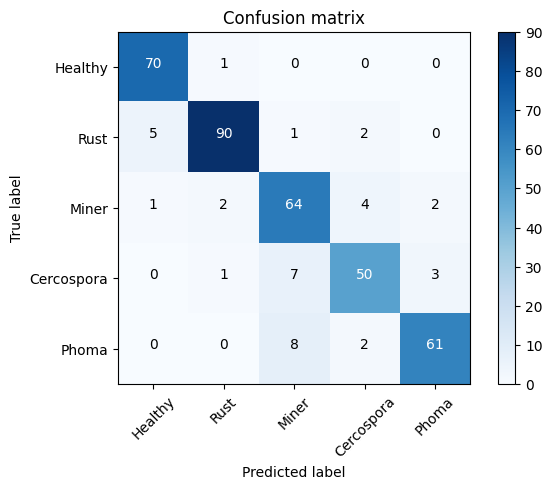
\includegraphics[scale = 0.5]{img/pavicnetV4.png}
            %\caption{Caption}
            \label{fig:enter-label}
        \end{figure}


        \column{0.5\textwidth}

        --------------- ACCURACY ----------------

        The accuracy for Healthy: 0.9813

        The accuracy for Rust: 0.9786

        The accuracy for Miner: 0.9358

        The accuracy for Cercospora: 0.9465

        The accuracy for Phoma: 0.9599

        Mean Accuracy:   0.9540

        --------------- PRECISION ----------------

        The precision for Healthy: 0.9211

        The precision for Rust: 0.9592

        The precision for Miner: 0.8025

        The precision for Cercospora: 0.8254

        The precision for Phoma: 0.8784

        Mean Precision: 0.8773

    \end{columns}
\end{frame}




% %---------------------------------------------------------



% %---------------------------------------------------------



\begin{frame}
    \frametitle{Próximos Passos}

    \begin{block}{Curto Prazo:}

        \begin{itemize}
            \item Pesquisar e definir novos datasets. \textsc{Concluído}
            \item Pré-Processar os novos datasets. \textsc{Concluído}
            \item \color{blue} Continuar o treinamento com o Dataset BRACOL.
        \end{itemize}

    \end{block}



    \begin{block}{Médio Prazo:}

        \begin{itemize}
            \item \color{blue} Iniciar o treinamento com os outros datasets.
            \item \color{blue} Dar continuidade a escrita do TCC.
        \end{itemize}

    \end{block}




\end{frame}


%------------------------------------------------------------------




% %---------------------------------------------------------



\begin{frame}
    \frametitle{Resultados preliminares}


    \centering

    \begin{figure}
        \centering
        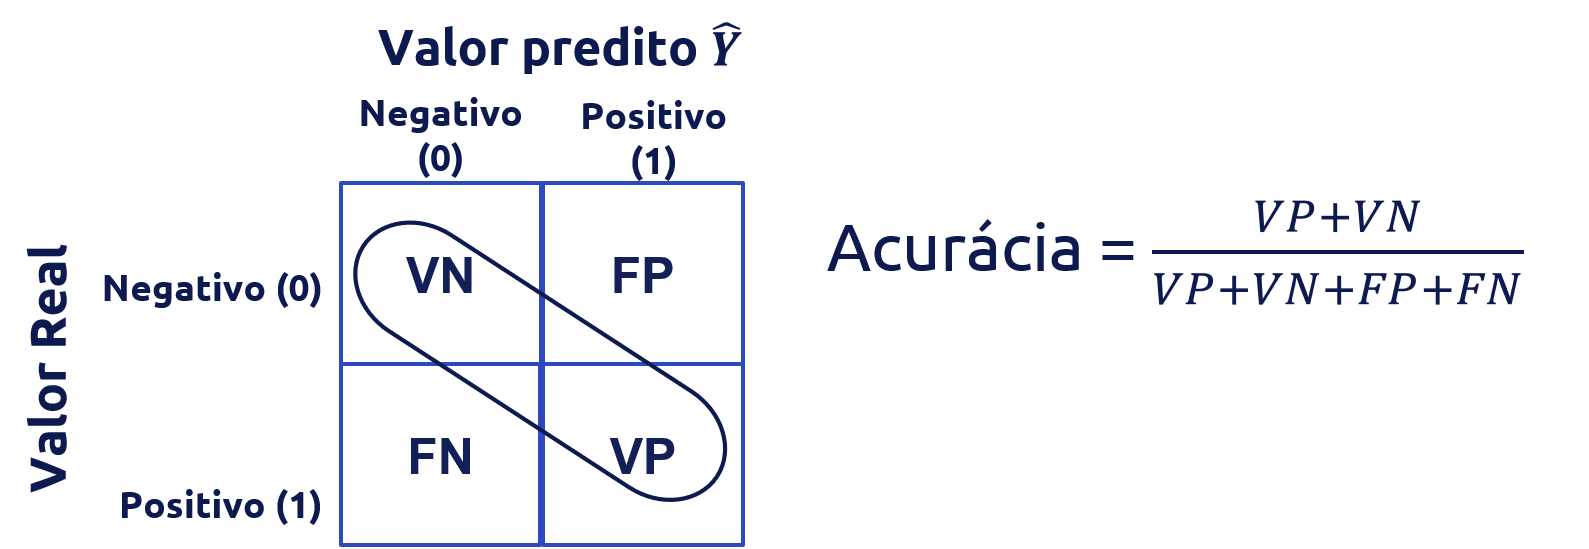
\includegraphics[scale = 0.5]{img/curacia.png}
        %\caption{Caption}
        \label{fig:enter-label}
    \end{figure}


\end{frame}




% %---------------------------------------------------------





% %---------------------------------------------------------



\begin{frame}
    \frametitle{Resultados preliminares}


    \centering

    \begin{figure}
        \centering
        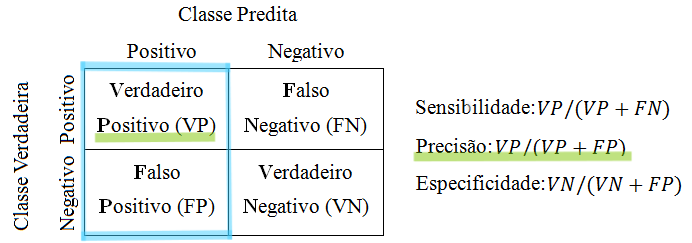
\includegraphics[scale = 0.7]{img/precisonmetric.png}
        %\caption{Caption}
        \label{fig:enter-label}
    \end{figure}


\end{frame}




% %---------------------------------------------------------



% %---------------------------------------------------------



\begin{frame}
    \frametitle{Resultados preliminares}

    \centering
    Acurácia

    \begin{figure}
        \centering
        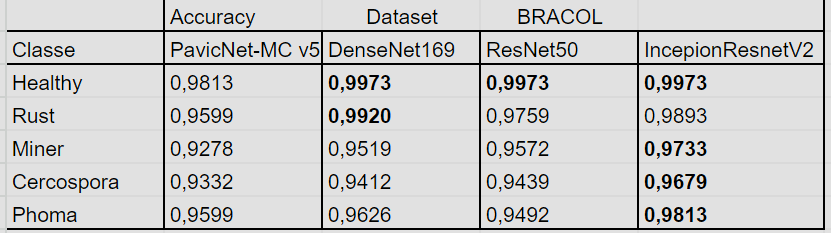
\includegraphics[scale = 0.7]{img/acc.png}
        %\caption{Caption}
        \label{fig:enter-label}
    \end{figure}



\end{frame}




% %---------------------------------------------------------




% %---------------------------------------------------------








% %---------------------------------------------------------


\begin{frame}
    \frametitle{Resultados preliminares}

    \centering
    Precisão

    \begin{figure}
        \centering
        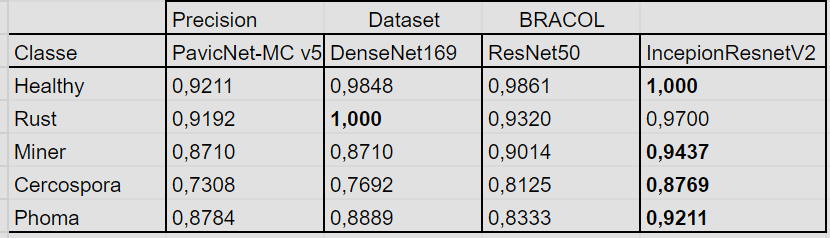
\includegraphics[scale = 0.7]{img/precision.png}
        %\caption{Caption}
        \label{fig:enter-label}
    \end{figure}



\end{frame}




% %---------------------------------------------------------



% %---------------------------------------------------------



\begin{frame}
    \frametitle{Resultados preliminares}


    \centering
    MobileNetV2


    \begin{columns}
        \column{0.5\textwidth}


        \begin{figure}
            \centering
            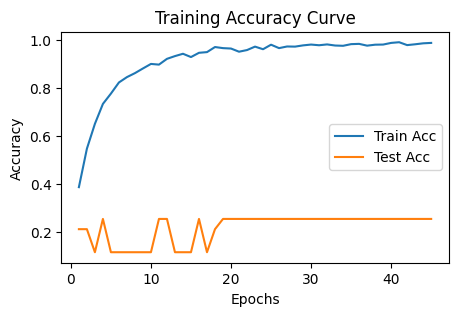
\includegraphics[scale = 0.5]{img/mobiletraincurve.png}
            %\caption{Caption}
            \label{fig:enter-label}
        \end{figure}


        \column{0.5\textwidth}


        \begin{figure}
            \centering
            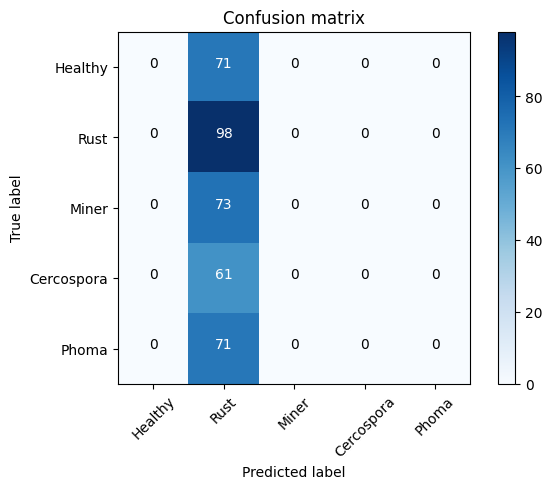
\includegraphics[scale = 0.5]{img/mobileresults.png}
            %\caption{Caption}
            \label{fig:enter-label}
        \end{figure}



    \end{columns}




\end{frame}




% %---------------------------------------------------------



% %---------------------------------------------------------



\begin{frame}
    \frametitle{Resultados preliminares}

    \begin{columns}


        \column{0.5\textwidth}

        \centering
        Training Set

        \begin{figure}
            \centering
            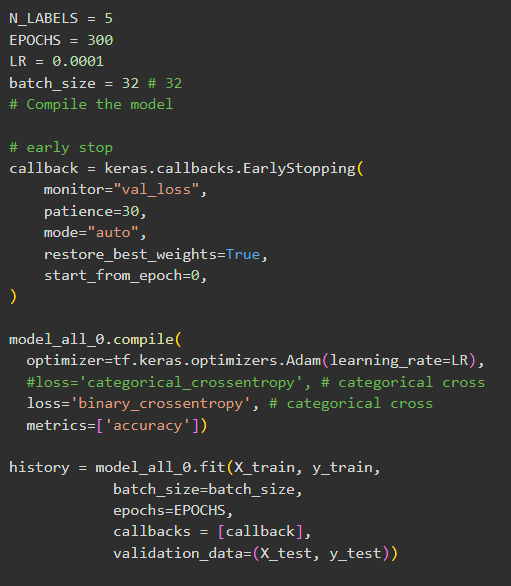
\includegraphics[scale = 0.4]{img/trainingSet.png}
            %\caption{Caption}
            \label{fig:enter-label}
        \end{figure}



        \column{0.5\textwidth}

        \centering
        MobileNetV2 config

        \begin{figure}
            \centering
            \includegraphics[scale = 0.4]{img/TmobileNet.png}
            %\caption{Caption}
            \label{fig:enter-label}
        \end{figure}



    \end{columns}





\end{frame}




% %---------------------------------------------------------



% %---------------------------------------------------------



\begin{frame}
    \frametitle{Próximos Passos}

    \begin{block}{Curto Prazo:}

        \begin{itemize}
            \item Pesquisar e definir novos datasets. \textsc{Concluído}
            \item Pré-Processar os novos datasets. \textsc{Concluído}
            \item Continuar o treinamento com o Dataset BRACOL.  \textsc{Concluído}
            \item \color{blue} Treinar com o dataset JMUBEN em RGB.
            \item \color{blue} Validar os resultados.
        \end{itemize}

    \end{block}



    \begin{block}{Médio Prazo:}

        \begin{itemize}
            \item \color{blue} Iniciar o treinamento com os outros datasets.
            \item \color{blue} Dar continuidade a escrita do TCC.
        \end{itemize}

    \end{block}




\end{frame}


%------------------------------------------------------------------

% %---------------------------------------------------------



\begin{frame}
    \frametitle{Próximos Passos}

    \begin{block}{Curto Prazo:}

        \begin{itemize}
            \item Pesquisar e definir novos datasets. \textsc{Concluído}
            \item Pré-Processar os novos datasets. \textsc{Concluído}
            \item Continuar o treinamento com o Dataset BRACOL.  \textsc{Concluído}
            \item Treinar com o dataset JMUBEN em RGB. \textsc{Concluído}
            \item Validar os resultados. \textsc{Concluído}
        \end{itemize}

    \end{block}



    \begin{block}{Médio Prazo:}

        \begin{itemize}
            \item \color{blue} Iniciar o treinamento com os outros datasets.
            \item \color{blue} Dar continuidade a escrita do TCC.
        \end{itemize}

    \end{block}




\end{frame}


%------------------------------------------------------------------




% %---------------------------------------------------------



\begin{frame}
    \frametitle{Resultados preliminares}

    \centering
    Acurácia - JMUBEN

    \begin{figure}
        \centering
        \includegraphics[scale = 0.7]{img/jmubenAcc.png}
        %\caption{Caption}
        \label{fig:enter-label}
    \end{figure}



\end{frame}




% %---------------------------------------------------------


% %---------------------------------------------------------



\begin{frame}
    \frametitle{Resultados preliminares}

    \centering
    Precisão - JMUBEN

    \begin{figure}
        \centering
        \includegraphics[scale = 0.7]{img/jmubenPrecs.png}
        %\caption{Caption}
        \label{fig:enter-label}
    \end{figure}



\end{frame}




% %---------------------------------------------------------




% %---------------------------------------------------------



\begin{frame}
    \frametitle{Resultados preliminares}


    \centering
    MobileNetV2


    \begin{columns}
        \column{0.5\textwidth}


        \begin{figure}
            \centering
            \includegraphics[scale = 0.5]{img/MobileTrain2.png}
            %\caption{Caption}
            \label{fig:enter-label}
        \end{figure}


        \column{0.5\textwidth}


        \begin{figure}
            \centering
            \includegraphics[scale = 0.5]{img/mobilematrix2.png}
            %\caption{Caption}
            \label{fig:enter-label}
        \end{figure}



    \end{columns}

\end{frame}




% %---------------------------------------------------------



% %---------------------------------------------------------



\begin{frame}
    \frametitle{Próximos Passos}

    \begin{block}{Curto Prazo:}

        \begin{itemize}
            \item Treinar com o dataset JMUBEN em RGB. \textsc{Concluído}
            \item Validar os resultados. \textsc{Concluído}
            \item \color{blue} Melhorar os resultados da PavicNet-MC.
            \item \color{blue} Implementar a arquitetura ShuffleNet.
            \item \color{blue} Pre-Processar os datasets RoCoLe e Diseases in coffe leafs.
        \end{itemize}

    \end{block}



    \begin{block}{Médio Prazo:}

        \begin{itemize}
            \item \color{blue} Iniciar o treinamento com dataset RoCoLe e DisCoLeafs.
            \item \color{blue} Dar continuidade a escrita do TCC.
        \end{itemize}

    \end{block}




\end{frame}


%------------------------------------------------------------------



% %---------------------------------------------------------


\begin{frame}
    \frametitle{Resultados preliminares}

    \centering
    Resultados de precisão de classificação de doenças e pragas nas folhas de café utilizando o dataset BRACOL.

    \begin{figure}
        \centering
        \includegraphics[scale = 0.7]{img/precision.png}
        %\caption{Caption}
        \label{fig:enter-label}
    \end{figure}



\end{frame}




% %---------------------------------------------------------




%---------------------------------------------------------

\begin{frame}
    \frametitle{Arquitetura PavicNet-MC}


    \begin{figure}
        \centering
        \includegraphics[scale=0.7]{img/pavicnet.png}
        %\caption{Caption}
        \label{fig:enter-label}
    \end{figure}


\end{frame}

%---------------------------------------------------------



\begin{frame}
    \frametitle{Arquitetura PavicNet-MC}


    \centering
    Convoluções nas imagens

    \begin{columns}
        \column{0.5\textwidth}


        \begin{figure}
            \centering
            \includegraphics[scale = 0.8]{img/convolutionGrid.png}
            %\caption{Caption}
            \label{fig:enter-label}
        \end{figure}


        \column{0.5\textwidth}


        \begin{figure}
            \centering
            \includegraphics[scale = 0.6]{img/Mapa de ativação.jpg}
            %\caption{Caption}
            \label{fig:enter-label}
        \end{figure}



    \end{columns}

\end{frame}



%---------------------------------------------------------

\begin{frame}
    \frametitle{Arquitetura PavicNet-MC}

    \centering
    Camada de MaxPooling
    (Camada de redução de dimensionalidade dos dados)

    \begin{figure}
        \centering
        \includegraphics[scale=0.4]{img/maxpooling.png}
        %\caption{Caption}
        \label{fig:enter-label}
    \end{figure}


\end{frame}

%---------------------------------------------------------




%---------------------------------------------------------

\begin{frame}
    \frametitle{Arquitetura PavicNet-MC}

    \vspace{-10px}
    \begin{columns}

        \column{0.3\textwidth}
        Nova PavicNet-MC:
        \begin{itemize}
            \item Modificações nas camadas de convolução e pooling
            \item Novas camadas de dropout
            \item De 755.989 para 519.173 parâmetros
        \end{itemize}

        \column{0.7\textwidth}

        \vspace{-30px}
        \begin{figure}
            \centering
            \includegraphics[scale=0.35]{img/NewPavicV7.png}
            %\caption{Caption}
            \label{fig:enter-label}
        \end{figure}


    \end{columns}




\end{frame}

%---------------------------------------------------------




%---------------------------------------------------------



\begin{frame}
    \frametitle{Arquitetura ShuffleNet}



    \begin{columns}


        \hspace{-30px}
        \column{0.5\textwidth}

        \vspace{-30px}
        \begin{figure}
            \centering
            \includegraphics[scale = 0.4]{img/shuffleunits.png}
            %\caption{Caption}
            \label{fig:enter-label}
        \end{figure}


        \column{0.5\textwidth}

        \vspace{-30px}
        \begin{figure}
            \centering
            \includegraphics[scale = 0.4]{img/shufflwMain.png}
            %\caption{Caption}
            \label{fig:enter-label}
        \end{figure}



    \end{columns}

\end{frame}



%---------------------------------------------------------






% %---------------------------------------------------------


\begin{frame}
    \frametitle{Resultados preliminares}

    \centering
    Novos resultados de precisão de classificação de doenças e pragas nas folhas de café utilizando o dataset BRACOL com a nova arquitetura PavicNet-MC e ShuffleNet implementadas.

    \begin{figure}
        \centering
        \includegraphics[scale = 0.62]{img/novosResultsPavicEShuffle.png}
        %\caption{Caption}
        \label{fig:enter-label}
    \end{figure}



\end{frame}




% %---------------------------------------------------------







%---------------------------------------------------------



\begin{frame}
    \frametitle{Resultados preliminares}



    \begin{columns}



        \column{0.5\textwidth}

        Importância da quantidade reduzida de parâmetros:
        \begin{itemize}
            \item Velocidade no treinamento do modelo
            \item Velocidade na classificação (utilização do modelo)
            \item Necessidade de um baixo custo computacional e memória (como dispositivos móveis, drones e etc)
        \end{itemize}

        \column{0.5\textwidth}

        \begin{figure}
            \centering
            \includegraphics[scale = 0.6]{img/drone é usado no monitoramento.jpg}
            %\caption{Caption}
            \label{fig:entelabel}
        \end{figure}


    \end{columns}

\end{frame}



%---------------------------------------------------------





% %---------------------------------------------------------



\begin{frame}
    \frametitle{Próximos Passos}

    \begin{block}{Curto Prazo:}

        \begin{itemize}
            \item Treinar com o dataset JMUBEN em RGB. \textsc{Concluído}
            \item Validar os resultados. \textsc{Concluído}
            \item Melhorar os resultados da PavicNet-MC. \textsc{Concluído}
            \item Implementar a arquitetura ShuffleNet. \textsc{Concluído}
            \item \color{blue} Pre-Processar os datasets RoCoLe e Diseases in coffe leafs.
        \end{itemize}

    \end{block}



    \begin{block}{Médio Prazo:}

        \begin{itemize}
            \item \color{blue} Iniciar o treinamento com dataset RoCoLe e DisCoLeafs.
            \item \color{blue} Dar continuidade a escrita do TCC.
        \end{itemize}

    \end{block}




\end{frame}


%------------------------------------------------------------------





\begin{frame}
    \frametitle{Resultados preliminares}



    \begin{columns}



        \column{0.5\textwidth}

        Diseases in Coffe Leaves (2021):
        \begin{itemize}
            \item 285 imagens da classe rust
            \item 257 imagens da classe miner
            \item Arquivo xml separado para cada imagem
        \end{itemize}

        \column{0.5\textwidth}

        \begin{figure}
            \centering
            \includegraphics[scale = 0.3]{img/diseasescanvas.png}
            %\caption{Caption}
            \label{fig:entelabel}
        \end{figure}


    \end{columns}

\end{frame}



%---------------------------------------------------------





%------------------------------------------------------------------





\begin{frame}
    \frametitle{Resultados preliminares}



    \begin{columns}



        \column{0.5\textwidth}

        RoCoLE (2019):
        \begin{itemize}
            \item 602 imagens da classe rust
            \item 791 imagens da classe healthy
            \item 167 imagens da classe red spider mite
            \item Diversos arquivos de marcação para todas as images (json, xml, xlsx, etc)
        \end{itemize}

        \column{0.5\textwidth}

        \begin{figure}
            \centering
            \includegraphics[scale = 0.05]{img/C4P20E2.jpg}
            %\caption{Caption}
            \label{fig:entelabel}
        \end{figure}


    \end{columns}

\end{frame}



%---------------------------------------------------------






% %---------------------------------------------------------



\begin{frame}
    \frametitle{Próximos Passos}

    \begin{block}{Curto Prazo:}

        \begin{itemize}
            \item Melhorar os resultados da PavicNet-MC. \textsc{Concluído}
            \item Implementar a arquitetura ShuffleNet. \textsc{Concluído}
            \item Pre-Processar o dataset RoCoLe. \textsc{Cancelado}
            \item \color{blue} Pre-Processar o dataset Diseases in coffe leafs.
        \end{itemize}

    \end{block}



    \begin{block}{Médio Prazo:}

        \begin{itemize}
            \item \color{blue} Iniciar o treinamento com o dataset DisCoLeafs.
            \item \color{blue} Iniciar treinamentos com o GPUFarm.
            \item \color{blue} Dar continuidade a escrita do TCC.
        \end{itemize}

    \end{block}




\end{frame}


%------------------------------------------------------------------





% %---------------------------------------------------------



\begin{frame}
    \frametitle{Resultados Preliminares}


    \begin{figure}
        \centering
        \includegraphics[scale = 0.3]{img/roboflow.png}
        %\caption{Caption}
        \label{fig:entelabel}
    \end{figure}




\end{frame}


%------------------------------------------------------------------


%------------------------------------------------------------------



\begin{frame}
    \frametitle{Resultados preliminares}


    \begin{columns}


        \column{0.5\textwidth}

        \begin{figure}
            \centering
            \includegraphics[scale = 0.3]{img/folhaRoboflow2.png}
            %\caption{Caption}
            \label{fig:entelabel}
        \end{figure}


        \column{0.5\textwidth}

        \begin{figure}
            \centering
            \includegraphics[scale = 0.3]{img/FolhRoboflow1.png}
            %\caption{Caption}
            \label{fig:entelabel}
        \end{figure}


    \end{columns}

\end{frame}


%---------------------------------------------------------



%------------------------------------------------------------------



\begin{frame}
    \frametitle{Resultados preliminares}


    \begin{columns}


        \column{0.4\textwidth}

        \begin{figure}
            \centering
            \includegraphics[scale = 0.35]{img/preprocessRoboflow.png}
            %\caption{Caption}
            \label{fig:entelabel}
        \end{figure}


        \column{0.6\textwidth}

        \begin{figure}
            \centering
            \includegraphics[scale = 0.35]{img/exportRRoboflow.png}
            %\caption{Caption}
            \label{fig:entelabel}
        \end{figure}


    \end{columns}

\end{frame}


%---------------------------------------------------------




% %---------------------------------------------------------



% \begin{frame}
% \frametitle{Resultados Preliminares}


% \begin{figure}
%     \centering
%     \includegraphics[scale = 0.3]{img/roboflow.png}
%     %\caption{Caption}
%     \label{fig:entelabel}
% \end{figure}




% \end{frame}


%------------------------------------------------------------------





% %---------------------------------------------------------



\begin{frame}
    \frametitle{Próximos Passos}

    \begin{block}{Curto Prazo:}

        \begin{itemize}
            \item Melhorar os resultados da PavicNet-MC. \textsc{Concluído}
            \item Implementar a arquitetura ShuffleNet. \textsc{Concluído}
            \item Pre-Processar o dataset RoCoLe. \textsc{Cancelado}
            \item Pre-Processar o dataset Diseases in coffe leafs. \textsc{Concluído}
            \item \color{blue} Converter o projeto de treinamento do Tensorflow para Pytorch.
        \end{itemize}

    \end{block}



    \begin{block}{Médio Prazo:}

        \begin{itemize}
            \item \color{blue} Iniciar o treinamento com o dataset DisCoLeafs.
            \item \color{blue} Iniciar treinamentos com o GPUFarm.
            \item \color{blue} Dar continuidade a escrita do TCC.
        \end{itemize}

    \end{block}




\end{frame}


%------------------------------------------------------------------














% %---------------------------------------------------------



\begin{frame}
    \frametitle{Resultados Preliminares}

    \centering

    \begin{figure}
        \centering
        \includegraphics[scale = 0.5]{img/imgprocess1.png}
        %\caption{Caption}
        \label{fig:entelabel}
    \end{figure}




\end{frame}


%------------------------------------------------------------------






% %---------------------------------------------------------



\begin{frame}
    \frametitle{Resultados Preliminares}

    \centering
    Resultados - Dataset: Diseases in coffee leaves DCL
    \begin{figure}
        \centering
        \includegraphics[scale = 0.7]{img/dlcResults.png}
        %\caption{Caption}
        \label{fig:entelabel}
    \end{figure}




\end{frame}


%------------------------------------------------------------------





% %---------------------------------------------------------



\begin{frame}
    \frametitle{Próximos Passos}

    \begin{block}{Curto Prazo:}

        \begin{itemize}
            \item Implementar a arquitetura ShuffleNet. \textsc{Concluído}
            \item Pre-Processar o dataset RoCoLe. \textsc{Cancelado}
            \item Pre-Processar o dataset Diseases in coffe leafs. \textsc{Concluído}
            \item \color{blue} Converter o projeto de treinamento do Tensorflow para Pytorch. \textsc{Em Andamento}
            \item \color{blue} Treinar modelos com os datasets mesclados.
        \end{itemize}

    \end{block}



    \begin{block}{Médio Prazo:}

        \begin{itemize}
            \item \color{blue} Dar inicio a escrita de artigo cientifico
            \item \color{blue} Dar continuidade a escrita do TCC.
        \end{itemize}

    \end{block}




\end{frame}


%------------------------------------------------------------------


\begin{frame}
    \frametitle{Próximos Passos}

    \begin{block}{Curto Prazo:}

        \begin{itemize}
            \item Finalizar a escrita da seção dos trabalhos relacionados.
            \item Escrever a seção de metodologia.


        \end{itemize}

    \end{block}



    \begin{block}{Médio Prazo:}

        \begin{itemize}
            \item \color{blue} Finzalizar a escrita de artigo cientifico
            \item \color{blue} Dar continuidade a escrita do TCC.
        \end{itemize}

    \end{block}




\end{frame}


%------------------------------------------------------------------



% IMAGEM DO ARTIGO

\begin{frame}
    \frametitle{Avanços: Escrita do artigo}

    \centering
    \begin{figure}
        \centering
        \includegraphics[scale = 0.5]{img/PrintArtigo.png}
        %\caption{Caption}
    \end{figure}


\end{frame}



%------------------------------------------------------------------


\begin{frame}
    \frametitle{Objetivo}

    \begin{columns}


        \column{0.5\textwidth}

        O objetivo deste trabalho é realizar uma detecção em duas etapas das doenças e pragas nas folhas de café. abordando tanto a identificação da região afetada pela doença quanto a classificação da doença especifica.


        \column{0.5\textwidth}
        \vspace{-0.5cm}
        \begin{figure}
            \centering
            \includegraphics[scale = 0.2]{img/folhaExemplloDetectada.jpg}
        \end{figure}


    \end{columns}

\end{frame}


%------------------------------------------------------------------



\begin{frame}
    \frametitle{Métodos}

    \centering
    \begin{figure}
        \centering
        \includegraphics[scale = 0.16]{img/fluxograma-2-estagios.png}
        %\caption{Caption}
    \end{figure}


\end{frame}



%------------------------------------------------------------------




\begin{frame}
    \frametitle{Métodos}

    \begin{columns}

        \column{0.5\textwidth}
        
        Modelos de detecção:
        \begin{itemize}
            \item YOLOv8
            \item YOLOv10
        \end{itemize}
        
        Modelos de classificação:
        \begin{itemize}
            \item DenseNet169
            \item InceptionResnetV2
            \item ShuffleNet
            \item ResNet50
        \end{itemize}


        \column{0.5\textwidth}

        Datasets utilizados
        \begin{itemize}
            \item BRACOL (1747 imagens)
            \item Diseases and Pests in Coffee Leaves (DPCL) (542 imagens)
        \end{itemize}
        
        Classes:
        \begin{itemize}
            \item Rust
            \item Miner
            \item Phoma
            \item Cercospora
            \item Healthy*
        \end{itemize}


    \end{columns}

\end{frame}





%---------------------------------------------------------



\begin{frame}
    \frametitle{Métodos}

    \centering
    \begin{figure}
        \centering
        \includegraphics[scale = 0.23]{img/ExemploDeteccao.png}
        %\caption{Caption}
    \end{figure}


\end{frame}


%---------------------------------------------------------



\begin{frame}
    \frametitle{Métodos}

    \centering
    \begin{figure}
        \centering
        \includegraphics[scale = 0.2]{img/ExemploClassificacao.png}
        %\caption{Caption}
    \end{figure}


\end{frame}


%---------------------------------------------------------


%------------------------------------------------------------------


\begin{frame}
    \frametitle{Próximos Passos}

    \begin{block}{Curto Prazo:}

        \begin{itemize}
            \item Finzalizar a sessão de Métodologia.
            \item Iniciar a sessão de resultados.


        \end{itemize}

    \end{block}



    \begin{block}{Médio Prazo:}

        \begin{itemize}
            \item \color{blue} Finzalizar a escrita de artigo cientifico
            \item \color{blue} Dar continuidade a escrita do TCC.
        \end{itemize}

    \end{block}




\end{frame}


%------------------------------------------------------------------





% \section{Second section}


% \begin{frame}
% \frametitle{Sample frame title}

% In this slide, some important text will be
% \alert{highlighted} because it's important.
% Please, don't abuse it.

% \begin{block}{Remark}
% Sample text
% \end{block}

% \begin{alertblock}{Important theorem}
% Sample text in red box
% \end{alertblock}

% \begin{examples}
% Sample text in green box. The title of the block is ``Examples".
% \end{examples}
% \end{frame}

% %---------------------------------------------------------


% %---------------------------------------------------------

% \begin{frame}
% \frametitle{Two-column slide}
% \begin{columns}

% \column{0.5\textwidth}
% This is a text in first column.
% $$E=mc^2$$

% \begin{itemize}
% \item First item
% \item Second item
% \end{itemize}

% \column{0.5\textwidth}
% This text will be in the second column
% and on a second tought this is a nice looking
% layout in some cases.

% \end{columns}
% \end{frame}

% %---------------------------------------------------------


\end{document}